% !TEX encoding = UTF-8 Unicode 
% !TEX root = praca.tex
\graphicspath{{chapters/chapter1/imgs/}}

\chapter{Narracja w grach}\label{chapter:ch1}

Niniejszy rozdział ma na celu dokonanie przeglądu gier komputerowych na przestrzeni lat, ze
szczególnym naciskiem na ewolucję sposobów oraz form narracji przedstawianych w tych grach.
Wyszczególnione zostaną również naistotniejsze struktury i rodzaje narracji, które są współcześnie
wykorzystywane. Dodatkowo, nastąpi krótki przegląd najpopularniejszych technik prezentacji narracji.
Na koniec nakreślone zostaną systemy dialogowe wykorzystywane przez gry komputerowe.

\section{Historia narracji w grach komputerowych}\label{section:ch1_1}

Aby zrozumieć istotę narracji w grach komputerowych, należy przede wszystkim określić
co może kryć się pod tym pojęciem. Pozwoli to dokonać przeglądu wybranych tytułów
i wyciągnąć z tego przeglądu wnioski. Żeby udowodnić rozwój w sposobie prezentowania narracji
na przestrzeni lat, prześledzone zostały części jednej z serii gier --- \textit{"Final Fantasy"} ---
wydawanej od roku 1987.

\subsection{Definicja narracji}\label{subsection:ch1_1_1}

Pojęcie narracji i samo jej występowanie w grach komputerowych jest kwestią sporną
w literaturze od lat. Barry Ip, w swojej pracy \cite{narrative_structures}, dokonuje wyróżnienia trzech słów ściśle
powiązanych ze sobą: \textit{historia}, \textit{fabuła} oraz \textit{narracja}. Na potrzeby jego
badań historia zdefiniowana została następująco:

\begin{quotation}
	\ldots \textit{sekwencja zdarzeń obejmujących byty.} \cite{narrative_structures}
\end{quotation}

Związana z historią jest również fabuła, która została określona przez Arystotelesa jako:

\begin{quotation}
	\ldots \textit{organizacja zdarzeń.} \cite{narrative_structures}
\end{quotation}

Sama narracja, ściśle powiązana z dwoma poprzednimi terminami, wyrażona została w sposób
następujący:

\begin{quotation}
	\ldots \textit{reprezentacja zdarzenia lub serii zdarzeń.} \cite{narrative_structures}
\end{quotation}

W ramach tej pracy, można przyjąć wszystkie te pojęcia jako istotne i na tyle bliskie
siebie, że mogą być wykorzystywane zamiennie.

Jakub Majewski sugeruje, że debatowanie nad istnieniem narracji jest odpowiednie dla niektórych
gier, a dla niektórych nie \cite{theorising_narrative}. Rozdzielenie bowiem tych form
przekazu, które można zaliczyć do treści fabularnej, nie jest takie oczywiste. Przytoczyć można
przykład \textit{Space Invaders} (1977) --- gra nie przytacza żadnego opisu w formie tekstowej,
skupiając się wyłącznie na rozgrywce. Na podstawie samego tytułu można jednak
przypuścić, że dokonuje się pewnego rodzaju inwazja, a stoją za nią przybysze z kosmosu \cite{theorising_narrative}.

Ten przykład pokazuje, że granica między grami posiadającymi narrację a tymi, w których jest ona nieobecna,
może być płynna. Nawet gry pozbawione bezpośrednich opisów fabularnych mogą zawierać pewne nawiązania narracyjne,
które wynikają z innych elementów, takich jak tytuł czy grafika. W związku z tym, podział na gry z narracją i bez
narracji może być problematyczny, ponieważ elementy narracyjne mogą przejawiać się w różnych formach i stopniach
w różnych grach. Jako że nie jest to główny problem poruszany w niniejszej pracy to wszystko co może być elementem
narracyjnym, jest za taki uznawany.

Do budowania narracji w grach wykorzystane mogą być wzorce znane z literatury. Przykładem takiego wzorca jest
\textit{"Podróż bohatera"}\cite{narrative_structures}, który opisuje 12 kluczowych etapów, odgrywających
istotną rolę w budowie angażujących historii (Tabela \ref{tab1:ch1_1_1}). Blisko powiązana z \textit{"Podróżą bohatera"}
jest znana struktura trzech aktów opisana przez Arystotelesa, która zakłada podział utworu na
początek, środek i koniec\cite{narrative_structures}. Jest to bardzo elastyczna a zarazem bardzo ogólna metoda
podziału. Zasadniczo w każdym utworze dałoby się bowiem w pewien sposób wyodrębnić te akty.

Struktury te pozwalają projektantom fabuły konstruować spójny świat fikcji --- niezależnie od formy w
jakiej zostanie zaprezentowana odbiorcom. Takowa może być adaptowana zarówno do powieści, jak i do materiału
filmowego czy też gier komputerowych.

\begin{table}[h!]
	\caption{Dwanaście etapów wzorca narracyjnego "Podróży bohatera" \cite{narrative_structures}}
	\label{tab1:ch1_1_1}
	\begin{center}
		\begin{tabular}{p{1.5in} p{4in}}
			\hline
			Etap                                & Opis                                                                                                                                                                                                                                                                                                                            \\
			\hline
			1. Zwyczajny świat                  & Gracz po raz pierwszy spotyka bohatera i zapoznaje się z jego pochodzeniem, zazwyczaj za pośrednictwem historii drugoplanowej                                                                                                                                                                                                   \\
			2. Wezwanie do przygody             & Wskazówka, że bohater opuści zwykły świat, by rozpocząć nową przygodę. Ten etap działa jak katalizator, który uruchamia główny wątek fabularny                                                                                                                                                                                  \\
			3. Odrzucenie wezwania              & W tradycyjnej strukturze monomitu bohater odrzuca początkową propozycję opuszczenia zwykłego świata i rozpoczęcia misji, zwykle w chwili wątpliwości lub niepewności                                                                                                                                                            \\
			4. Spotkanie z mentorem             & Gdy bohater decyduje się na podjęcie zadania, mentor dostarcza mu informacji potrzebnych do podjęcia decyzji. Mentorem może być wszystko, co dostarcza informacji - brodaty starzec, robot, biblioteka, doświadczenia z przeszłości i tak dalej                                                                                 \\
			5. Przekroczenie pierwszego progu   & Bohater przechodzi z bezpiecznego zwykłego świata do nowego, niebezpiecznego i nieznanego świata poszukiwań                                                                                                                                                                                                                     \\
			6. Testy, sprzymierzeńcy i wrogowie & Faza ta jest zwykle największą częścią fabuły gry, ponieważ gracz poznaje wszystkie główne postacie                                                                                                                                                                                                                             \\
			7. Podejście do najgłębszej jaskini & Jest to miejsce, w którym bohater znajduje nagrodę, której szuka - taką jak zdobycie niezbędnej umiejętności, broni lub opanowanie wszystkiego, co napotkał do tej pory. Zazwyczaj ma to miejsce pod koniec gry. Głównym celem tej części historii jest przygotowanie bohatera do ostatecznej bitwy                             \\
			8. Próba                            & To tutaj bohater staje do ostatecznej walki ze swoim nemezis lub "ostatecznym bossem". Nemezis może pojawić się jako byt fizyczny (osoba lub przedmiot) lub niefizyczny (czas, intensywność lub trudność)                                                                                                                       \\
			9. Nagroda                          & Wiele gier kończy się w tym momencie, gdy wróg zostaje pokonany, a nagrodą jest zazwyczaj końcowa cut-scenka opisująca, co dzieje się z bohaterem po jego triumfie                                                                                                                                                              \\
			10. Droga powrotna                  & Niektóre gry pozwolą graczowi powrócić do zwykłego świata po otrzymaniu nagrody, ale może nie być możliwe, aby bohater z powodzeniem zintegrował się ze starym światem                                                                                                                                                          \\
			11. Wksrzeszenie                    & Ta część historii odpowiada na wszelkie pytania bez odpowiedzi, takie jak konsekwencje misji, potencjalne konflikty, które mogą pojawić się w przyszłych sequelach, lub wszelkie testy, którym bohater musi stawić czoła przed końcem. Może mieć również formę ostatecznego zwrotu akcji, jako coś nieoczekiwanego przez widzów \\
			12. Powrót z nagrodą                & Jest to ostatni etap historii, w którym bohater w końcu powraca do zwykłego świata i widzi korzyści płynące z jej nagrody. Bohater może porównać swoje życie przed i po wyprawie, aby zobaczyć, jak wszystko się zmieniło                                                                                                       \\
			\hline
		\end{tabular}
	\end{center}
\end{table}

\newpage

\subsection{Przedstawienie narracji w grach na przestrzeni lat}\label{subsection:ch1_1_2}

Kamienie milowe w początkach branży gier wideo to: Spacewar (Rys \ref{fig:ch1_1_2_spacewar}) - pierwsza interaktywna gra z
1962 roku, Magnavox Odyssey (1972) - pierwszy domowy system gier podłączany do telewizora, a
także Pong (Rys \ref{fig:ch1_1_2_pong}) od Atari (1972) i przenośne gry LED Mattela (1977)\cite{the_evolution_of_video_games}.

Gra "Spacewar" (Rys \ref{fig:ch1_1_2_spacewar}) przedstawia dwa statki kosmiczne, które w obrębie studni potencjału grawitacyjnego ("gravity well")
prowadzą ze sobą starcie. Jeden ze statków nazywany jest "igłą" a drugi "klinem". Oba są sterowane przez
graczy, którzy mają do dostępu ograniczoną amunicję i paliwo do nawigowania. Cała rozgrywka prowadzona jest
na planszy 2-wymiarowej, gdzie tło stanowią gwiazdy. Gra nie posiada żadnej formy narracji, natomiast była
istotnym elementem dalszego rozwoju branży.

\begin{figure}[h]
	\caption{Spacewar (1962)}
	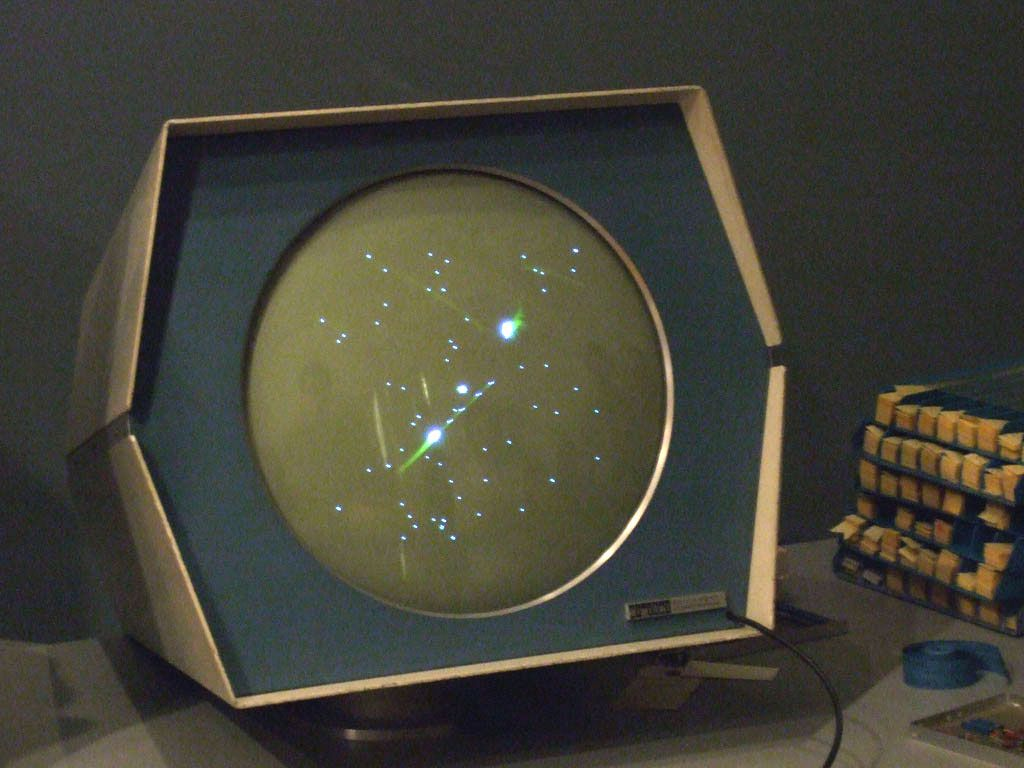
\includegraphics[width=0.5\textwidth]{ch1_1_2_spacewar.jpg}
	\centering
	\label{fig:ch1_1_2_spacewar}
\end{figure}

W ramach rozgrywki w "Pong" (Rys \ref{fig:ch1_1_2_pong}) mamy do czynienia z symulatorem tenisa stołowego. Dwójka graczy steruje paletkami
poruszającymi się pionowo. Za pomocą tych paletek odbijają piłkę na stronę przeciwnika. Jeśli ten nie odbije
jej z powrotem, to uderzający zdobywa punkt. Wygrywa pierwszy gracz, który uzyska 11 punktów. Podobnie jak
w przypadku "Spacewar", "Pong" nastawiony jest na rozgrywkę dwuosobową i nie posiada żadnej formy narracji.

\begin{figure}[h]
	\caption{Pong (1972)}
	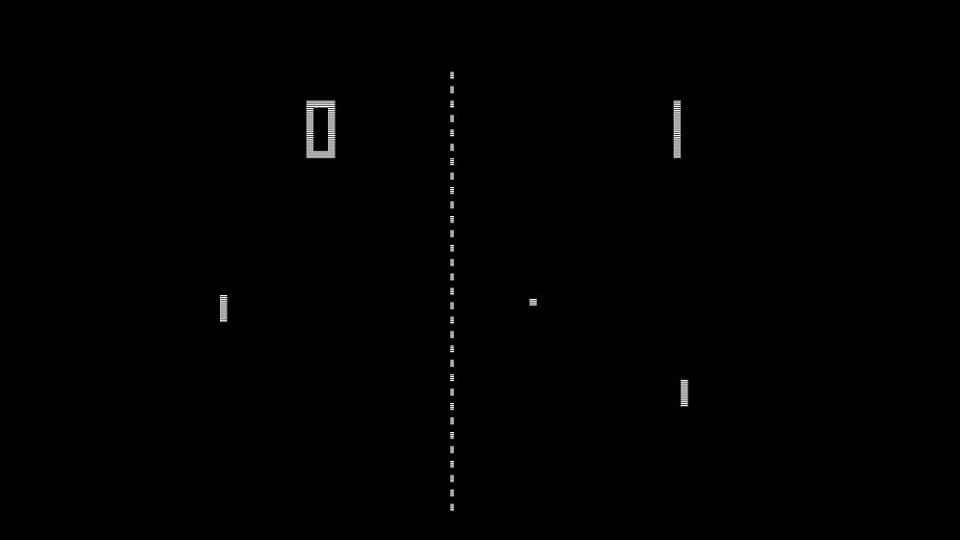
\includegraphics[width=0.5\textwidth]{ch_1_1_2_pong.jpg}
	\centering
	\label{fig:ch1_1_2_pong}
\end{figure}

Lata 70. przyniosły rozwój firm jak Atari, Nintendo i Sega oraz pierwsze hity salonów
gier np. Pacman (1980), który sprzedał 300 000 sztuk na całym świecie\cite{the_evolution_of_video_games}.

W "Breakout" (Rys \ref{fig:ch1_1_2_breakout}) gracz steruje paletką poruszającą się poziomo i stara się zniszczyć położoną wyżej ścianę
z cegiełek. Ściana składa się z ośmiu rzędów kolorowych bloczków. Używając pojedynczej piłki należy
zbić jak najwięcej cegiełek (przy kontakcie piłki z cegiełką zostaje ona zniszczona). Grający posiada
trzy życia i w ramach nich musi wyczyścić dwie ściany. Gracz traci życie jeśli nie odbije piłki wracającej
do niego. Rozgrywka ta została zaplanowana na maszyny \textit{arcade} z myślą o zdobywaniu jak najwięcej
punktów. Nie da się dostrzec w jej przypadku żadnej formy fabuły.

\begin{figure}[h]
	\caption{Breakout (1976)}
	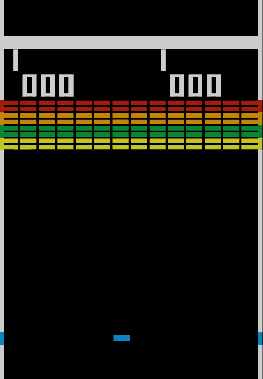
\includegraphics[width=0.5\textwidth]{ch1_1_2_breakout.jpg}
	\centering
	\label{fig:ch1_1_2_breakout}
\end{figure}

"Space Invaders" (Rys \ref{fig:ch1_1_2_space_invaders}) to gra akcji opracowana i wydana w Japonii przez Taito. Gracz steruje działem laserowym
umieszczonym na dole ekranu, które porusza się poziomo. Kosmici ułożeni w 5 rzędów po 11 obiektów
przemieszczają się grupowo w lewo i prawo, schodząc niżej gdy dotkną krawędzi ekranu. Celem gry jest
zestrzelenie wszystkich kosmitów przez gracza, posiadającego trzy życia. Obcy wystrzeliwują swoje pociski,
które przy trafieniu w gracza zabierają mu jedno życie. Gra kończy się natychmiastowo w momencie gdy
najeźdźcy dotrą do dołu ekranu. Tak jak w przypadku "Breakout" mamy do czynienia z rozgrywką nastawioną na
maszyny \textit{arcade}, a co za tym idzie na zdobywanie punktów. Oprócz kwestii poruszanych w
podsekcji \ref{subsection:ch1_1_1}, nie występują inne przesłanki fabularne.

\begin{figure}[h]
	\caption{Space Invaders (1978)}
	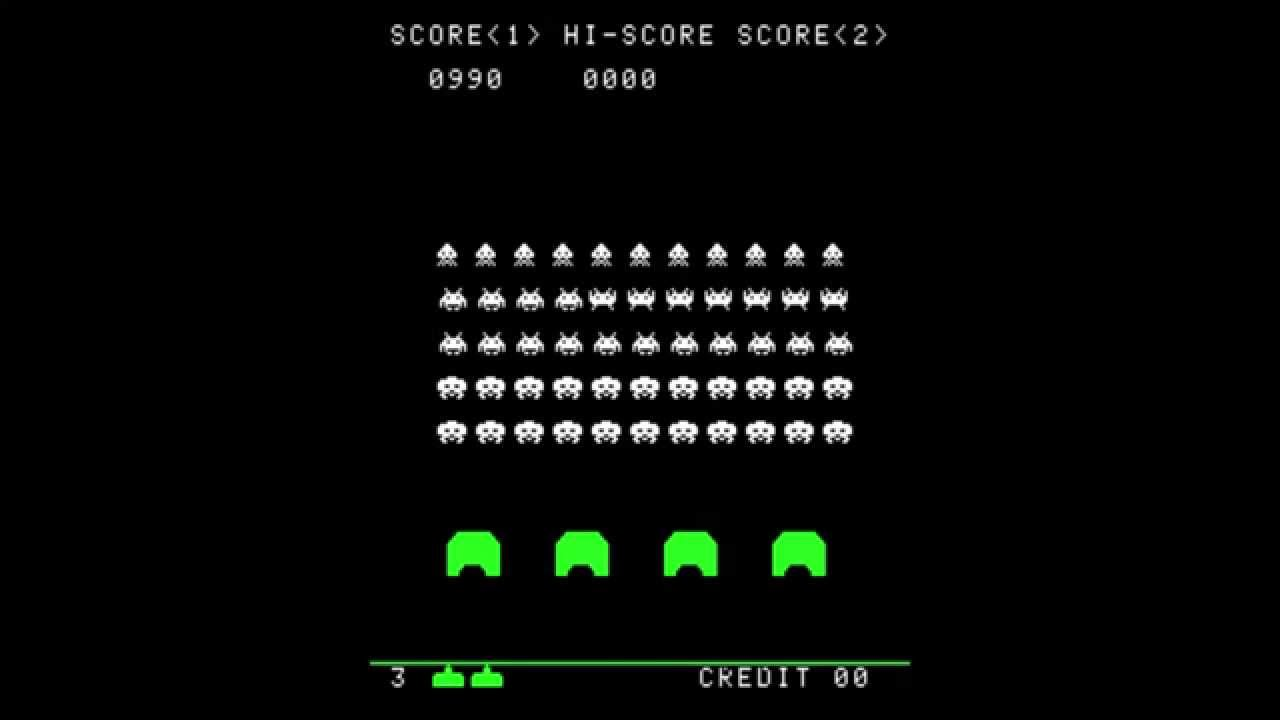
\includegraphics[width=0.5\textwidth]{ch_1_1_2_space_invaders.jpg}
	\centering
	\label{fig:ch1_1_2_space_invaders}
\end{figure}

\newpage

W latach 80. nastąpił boom konsol domowych - Nintendo NES, Sega Master System, Atari 7800\cite{the_evolution_of_video_games}.
Obecnie kiedy większość graczy myśli o grach \textit{retro} to ma na myśli między innymi właśnie tytuły
wyprodukwane na te serie konsol.

Jedną z najbardziej znanych w popkulturze gier jest "Super Mario Bros." (Rys \ref{fig:ch1_1_2_super_mario_bros}).
Gracz wciela się w rolę tytułowego Mario (w wersji jednoosobowej), który ma jako główne zadanie obrane
ocalenie księżniczki. W tym celu pokonuje kolejne krainy (poziomy) oraz przeciwników. Gra składa się z ośmiu
światów, gdzie każdy z nich jest dodatkowo podzielony na cztery poziomy. Mamy więc do czynienia z
wielopoziomową formą rozrywki, gdzie światy różnią się między sobą ze względu na warstwę wizualną, dźwiękową
jak i ze względu na występujących przeciwników czy przeszkody. Są to pewnego rodzaju zalążki narracji
(która została wykreowana przez świat). Jedyną formą pisemnej fabuły jest tekst występujący po ukończeniu
poziomu (Rys \ref{subfig:ch_1_1_2_mario_2}).

\begin{figure}[h]
	\begin{subfigure}{0.49\textwidth}
		\caption{Ekran tytułowy}
		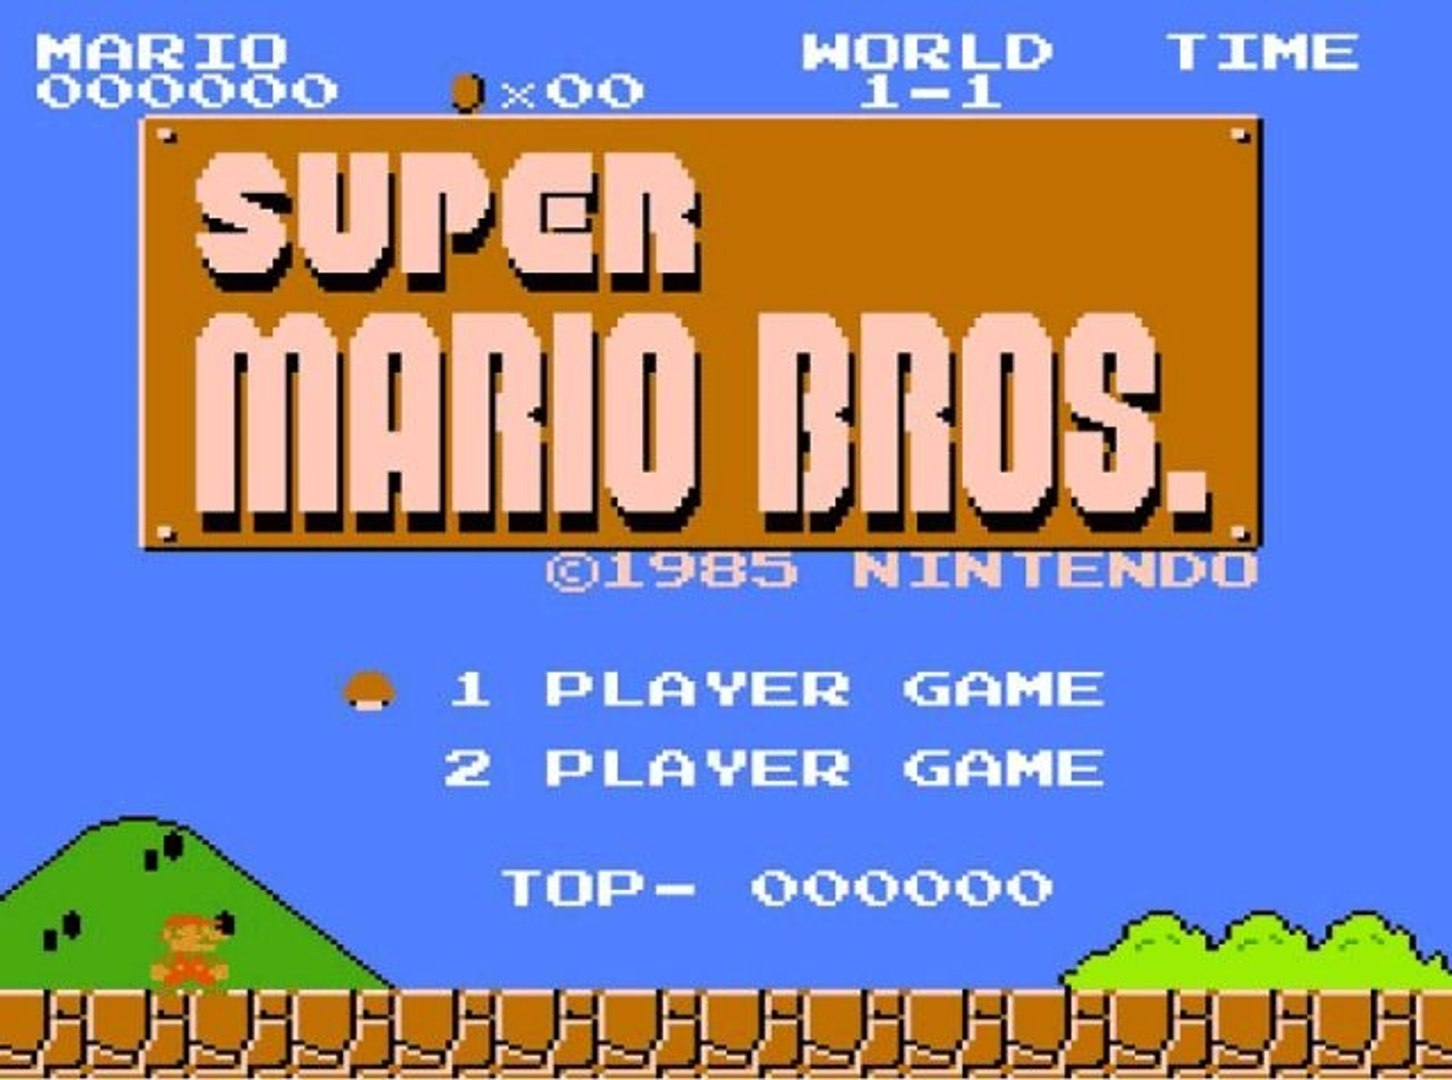
\includegraphics[width=\linewidth, height=6cm]{ch_1_1_2_mario_1.jpg}
		\label{subfig:ch_1_1_2_mario_1}
	\end{subfigure}
	\begin{subfigure}{0.49\textwidth}
		\caption{Ukończenie poziomu}
		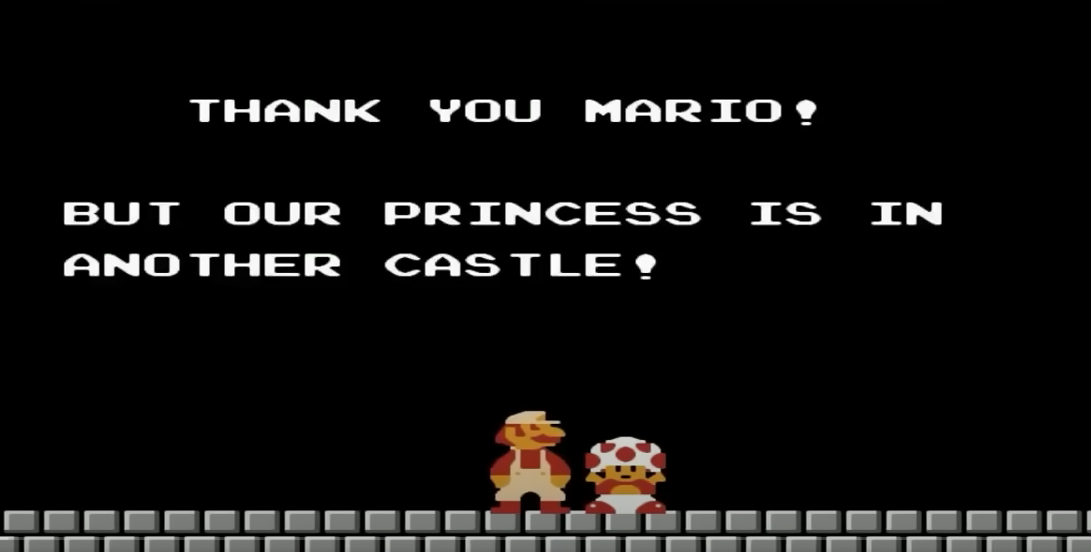
\includegraphics[width=\linewidth, height=6cm]{ch_1_1_2_mario_2.png}
		\label{subfig:ch_1_1_2_mario_2}
	\end{subfigure}
	\caption{Super Mario Bros. (1985)}
	\label{fig:ch1_1_2_super_mario_bros}
\end{figure}

"The Legend of Zelda" (Rys \ref{fig:ch1_1_2_zelda}) to gra przygodowa, w której główną postacią sterowaną
przez gracza jest Link. Jego zadaniem jest zebranie ośmiu fragmentów Trójkątnej wiedzy
(ang. \textit{Triforce of Wisdom}) by uratować księżniczkę Zeldę. Przy rozpoczęciu rozgrywki graczowi
przedstawiany jest ekran ze wstępem fabularnym (Rys \ref{subfig:ch_1_1_2_zelda_1}). Gra posiadała
również dedykowaną instrukcję, która na zasadzie poradnika podawała wskazówki dotyczące rozgrywki.
Tak jak w przypadku "Super Mario Bros.", występuje podział na poziomy, a co za tym idzie zmienia się
oprawa audio-wizualna jak i spotykani przeciwnicy. W trakcie rozgrywki możemy napotkać na postacie
NPC (ang. \textit{non-playable character}), które komunikują się za pomocą krótkiego stwierdzenia
(Rys \ref{subfig:ch_1_1_2_zelda_2}). Widoczne są również zalążki motywu "otwartego świata", gdzie gracz
zwiedza świat i jego elementy w dowolnej kolejności.

\begin{figure}[h]
	\begin{subfigure}{0.49\textwidth}
		\caption{Wstęp fabularny}
		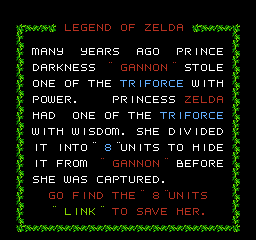
\includegraphics[width=\linewidth, height=6cm]{ch_1_1_2_zelda_1.png}
		\label{subfig:ch_1_1_2_zelda_1}
	\end{subfigure}
	\begin{subfigure}{0.49\textwidth}
		\caption{Interakcja z NPC}
		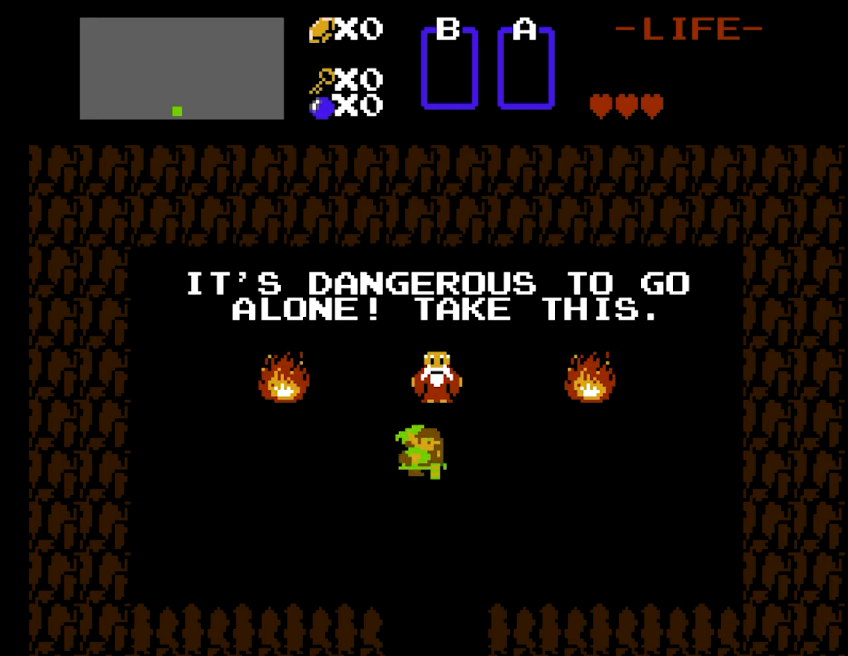
\includegraphics[width=\linewidth, height=6cm]{ch_1_1_2_zelda_2.png}
		\label{subfig:ch_1_1_2_zelda_2}
	\end{subfigure}
	\caption{The Legend of Zelda (1986)}
	\label{fig:ch1_1_2_zelda}
\end{figure}

Dekadę później gry komputerowe PC zyskały popularność dzięki tytułom jak Doom, a na rynku
pojawiły się PlayStation i Nintendo 64. Koniec XX wieku to także rozwój przenośnych gier na
fali sukcesu serii Pokemon.

Pierwszym tytułem opisanym w tej podsekcji, który operuje na perspektywie 3-osobowej jest
"Crash Bandicoot" (Rys \ref{fig:ch1_1_2_crash}). W wydanej na platformę PlayStation w 1996 roku grze
gracz steruje tytułowym Crash'em Bandicoot'em. Rozgrywkę otwiera tzw. cut-scenka (wyjaśniona również w
podsekcji \ref{subsection:ch1_2_3}), czyli krótki film wprowadzający do fabuły. To właśnie dzięki niej
gracz może usłyszeć wypowiadane imię głównego przeciwnika Crasha, doktora Neo Cortex'a.
Szalony naukowiec prowadził badania na lokalnej faunie i pragnął by Crash
stał się generałem jego armii. Crash zostaje jednak odrzucony przez maszynę do prania mózgu i ucieka
z zamku Cortex'a. Pod koniec filmu przedstawiona zostaje też "kobieta Bandicoot", na której mają zostać
przeprowadzone dalsze testy. W ten sposób gracz odkrywa dlaczego Crash przemierza kolejne poziomy (by ocalić
panią Bandicoot), dlaczego przeciwnicy są tacy a nie inni (przez testy doktora Neo Cortex'a) i co za tym
idzie kto jest jego głównym rywalem. Dodatkowo, w ramach rozgrywki mamy do czynienia z perspektywą
trójwymiarową, która jednak ulega zmianie pomiędzy poziomami. W grze występują również dwa zakończenia,
jedno wymaga perfekcyjnego przejścia gry, natomiast oba przedstawione są w formie cut-scenki.

\begin{figure}[h]
	\begin{subfigure}{0.49\textwidth}
		\caption{Cut-scenka otwierająca}
		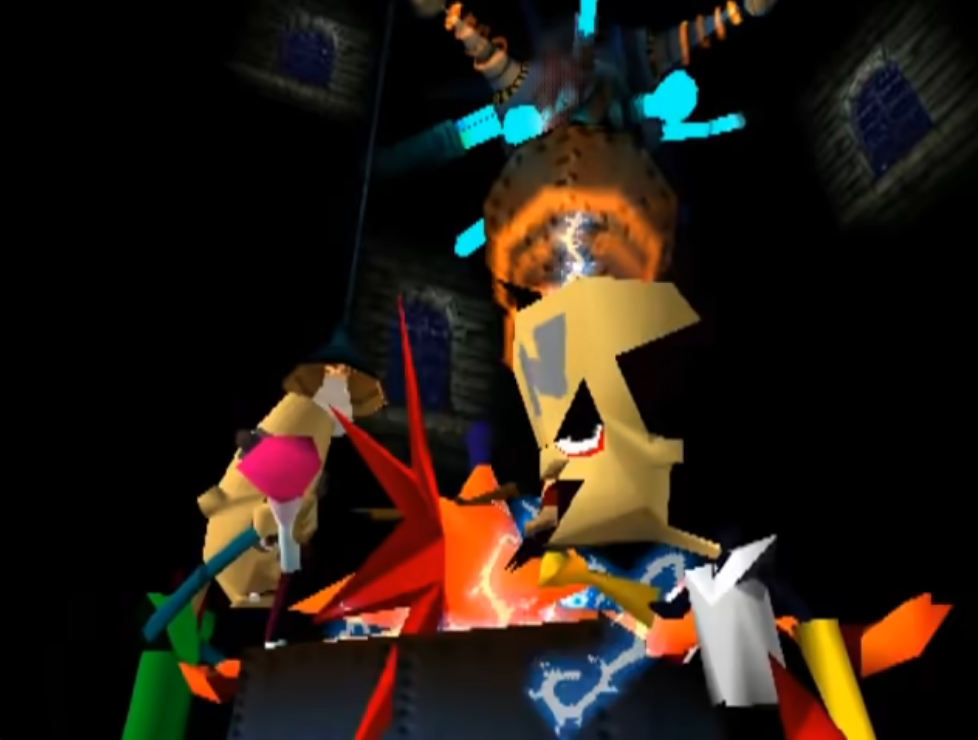
\includegraphics[width=\linewidth, height=6cm]{ch_1_1_2_crash_1.png}
		\label{subfig:ch_1_1_2_crash_1}
	\end{subfigure}
	\begin{subfigure}{0.49\textwidth}
		\caption{Crash i jego towarzysz Aku Aku}
		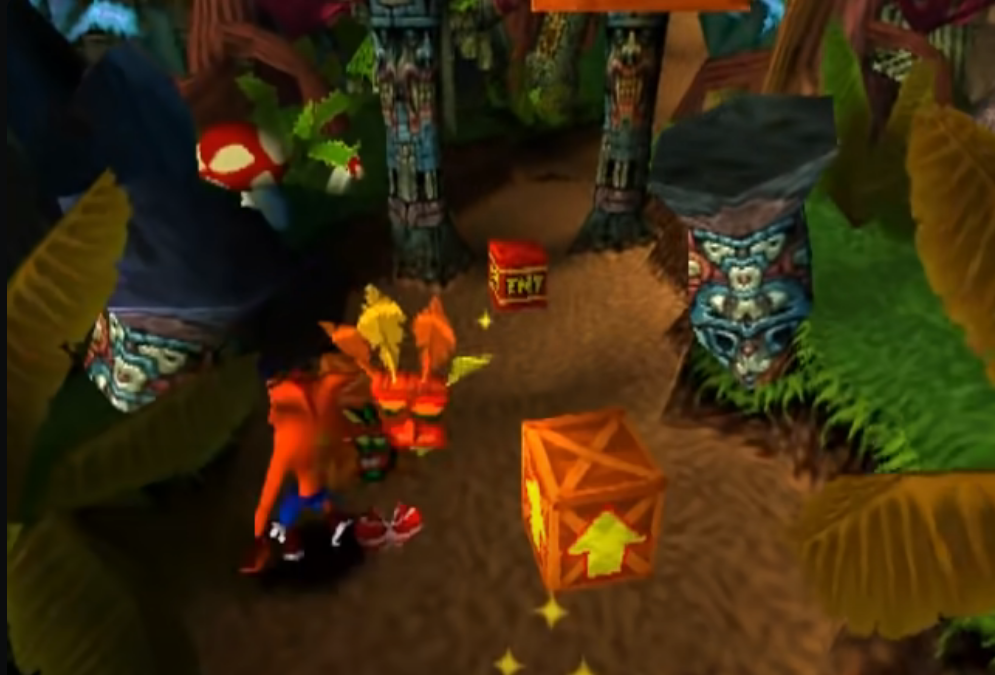
\includegraphics[width=\linewidth, height=6cm]{ch_1_1_2_crash_2.png}
		\label{subfig:ch_1_1_2_crash_2}
	\end{subfigure}
	\caption{Crash Bandicoot (1996)}
	\label{fig:ch1_1_2_crash}
\end{figure}

Uznawaną za jedną z najlepszych czy też najbardziej kultowych gier komputerowych jest
"Half-Life" (Rys \ref{fig:ch1_1_2_hl}) wydany w 1998 roku.
Wprowadzająca do rozgrywki sekwencja przedstawia najważniejsze informacje, nie zabierając
przy tym kontroli (gracz może przemieszczać się i rozglądać po kabinie pociągu). Nakreślona zostaje
postać Gordona Freemana, 27-letniego doktora fizyki teoretycznej, który pracuje w placówce Black Mesa,
położonej w Nowym Meksyku. Niemal cała warstwa fabularna zostaje wypowiedziana przez aktorów głosowych,
bez wspierających napisów. Gracz w trakcie rozgrywki spotyka różnych NPC - i to właśnie one
przekazują mu istotne informacje (posiadają również odpowiednie animacja poruszania ustami przy
wypowiadaniu kwestii). Przejścia pomiędzy poziomami są maskowane przez m.in. podróże windą czy
bardzo krótkie doczytywanie kolejnych fragmentów świata --- co sprawia, że rozgrywka pozostaje
bez przerwy imersyjna.

\begin{figure}[h]
	\begin{subfigure}{0.49\textwidth}
		\caption{NPC w monologu}
		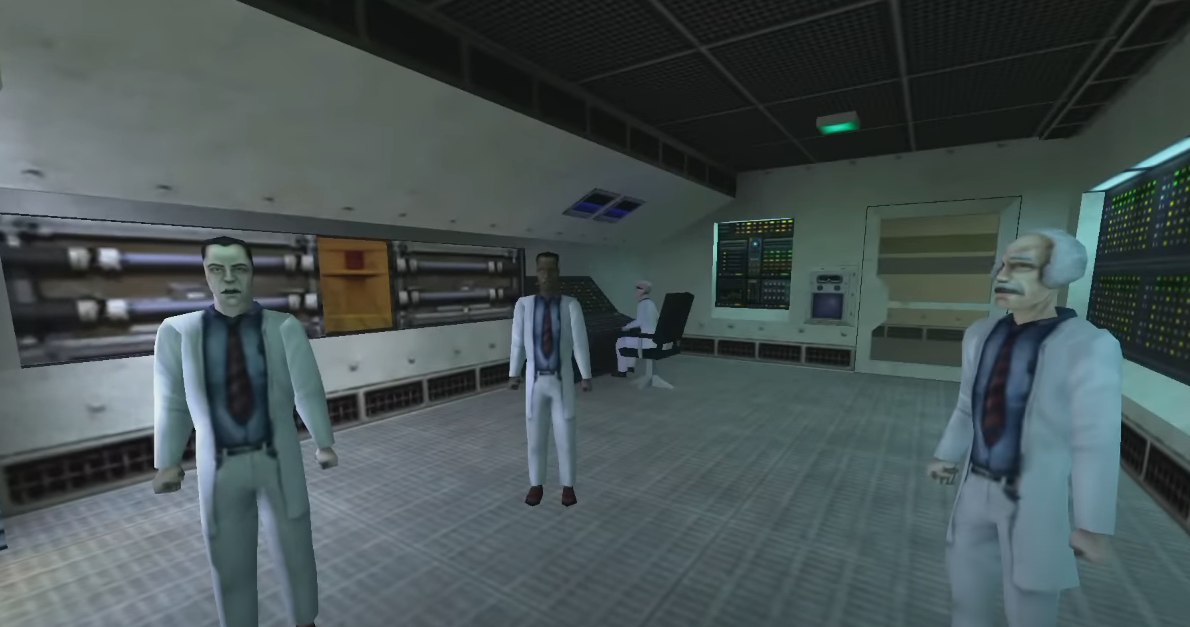
\includegraphics[width=\linewidth, height=6cm]{ch_1_1_2_hl_1.png}
		\label{subfig:ch_1_1_2_hl_1}
	\end{subfigure}
	\begin{subfigure}{0.49\textwidth}
		\caption{Napisy w sekwencji otwierającej}
		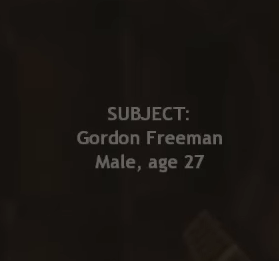
\includegraphics[width=\linewidth, height=6cm]{ch_1_1_2_hl_2.png}
		\label{subfig:ch_1_1_2_hl_2}
	\end{subfigure}
	\caption{Half-life (1998)}
	\label{fig:ch1_1_2_hl}
\end{figure}

\newpage

Nowe millennium przyniosło dalszy rozwój branży do rozmiarów dzisiejszej potęgi, poprzez stale
pojawiające się innowacje sprzętowe i nowe przełomowe tytuły na różne platformy.

Przykładem idealnie obrazującym rozwój w podejściu do narracji jest gra "Life is Strange" (Rys \ref{fig:ch1_1_2_lis})
wydana w 2015 roku. Jest to gra przygodowa o charakterze fikcji interkatywnej (Więcej na ten temat
w podsekcji \ref{subsection:ch1_3_2}), która wydawana była w formie epizodycznej. Każdy epizod
przypominać może podział na odcinki znany z seriali telewizyjnych czy też akty w literaturze.
Centralną postacią jest Maxine Caulfield, która odkrywa że potrafi cofnąć czas. Całość fabuły opiera się
na motywie \textit{efektu motyla}, gdzie podejmowane decyzje mogą rzutować na wydarzenia w przyszłości czy
też na relacje pomiędzy postaciami. Z tego powodu narrację można zakwalifikować jako rozgałęziającą się
(Patrz \ref{subsection:ch1_2_1}) i zarazem stanowi ona kluczowy element rozgrywki a nie tylko
"imersyjny dodatek" do niej. System dialogów zaprezentowany w "Life is Strange" oparty jest na popularnej
strukturze kołowej (Patrz \ref{subsection:ch1_3_1}) z motywem drzewa, tzn. konkretne wybory dialogowe
wiążą się z gamą zupełnie nowych wyborów w dalszej części rozmowy (mechanika cofania czasu pozwala
graczowi rozgrywać dialog na inny sposób).

\begin{figure}[h]
	\begin{subfigure}{0.49\textwidth}
		\caption{Wybór z ostrzeżeniem o konsekwencjach}
		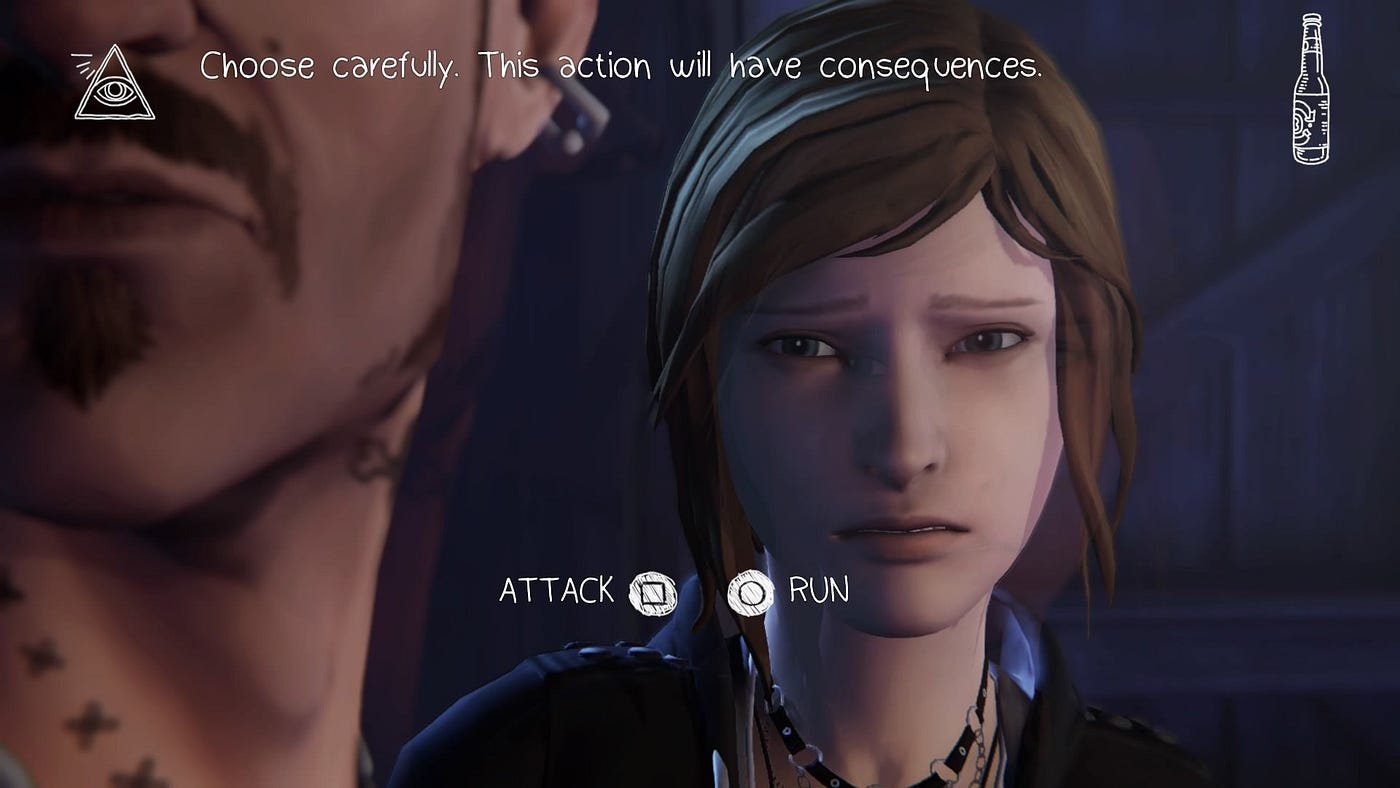
\includegraphics[width=\linewidth, height=6cm]{ch_1_1_2_lis_1.png}
		\label{subfig:ch_1_1_2_lis_1}
	\end{subfigure}
	\begin{subfigure}{0.49\textwidth}
		\caption{System dialogowy kołowy}
		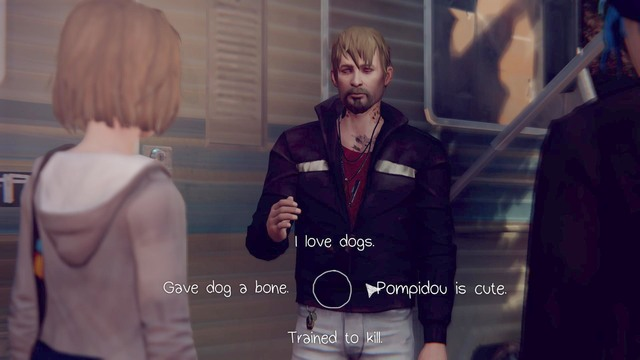
\includegraphics[width=\linewidth, height=6cm]{ch_1_1_2_lis_2.png}
		\label{subfig:ch_1_1_2_lis_2}
	\end{subfigure}
	\caption{Life is Strange (2015)}
	\label{fig:ch1_1_2_lis}
\end{figure}

\newpage

Jako wzór gry z otwartym światem niewątpliwie można uznać tytuł "Wiedźmin 3" (Rys \ref{fig:ch1_1_2_witcher})
wydane w 2015 roku i wyprodukowane przez polskie studio CD Projekt Red. Akcja rozgrywka się w świecie
opartym na powieściach i opowiadaniach Andrzeja Sapkowskiego a gracz wciela się w rolę Geralta z Rivii.
Forma otwartego świata oznacza w tym przypadku tyle, że grający ma możliwość swobodnego poruszania się
po krainach i jest też w stanie podejmować się różnych zadań w "niemal" dowolnej kolejności. Sprawia to, że
gracz nie czuje się niczym aktor odgrywający kolejne sceny a za to jest reżyserem własnych przygód.
System dialogowy zorganizowany jest w formę menu wyborów, przy czym na niektóre zdarzenia gracz ma
ograniczony czas odpowiedzi (Przedstawione na Rys. \ref{subfig:ch_1_1_2_witcher_2}). Dodatkowo, niektóre
opcje mogą wymagać posiadania określonej ilości pieniędzy czy też odblokowania określonych umiejętności.

\begin{figure}[h]
	\begin{subfigure}{0.49\textwidth}
		\caption{Mapa świata (żółte punkty - zadania)}
		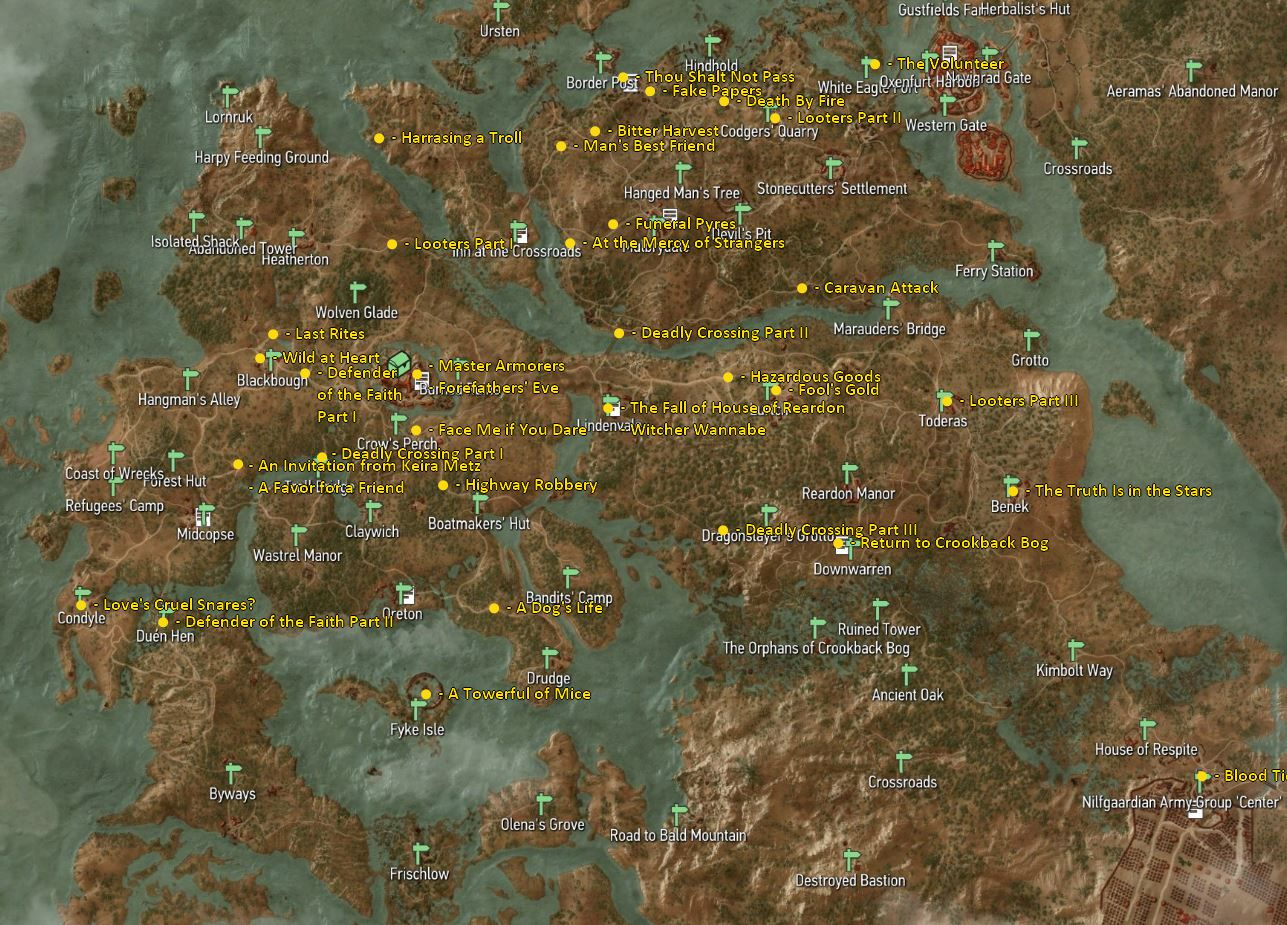
\includegraphics[width=\linewidth, height=6cm]{ch_1_1_2_witcher_1.png}
		\label{subfig:ch_1_1_2_witcher_1}
	\end{subfigure}
	\begin{subfigure}{0.49\textwidth}
		\caption{Dialog z czasem na decyzję}
		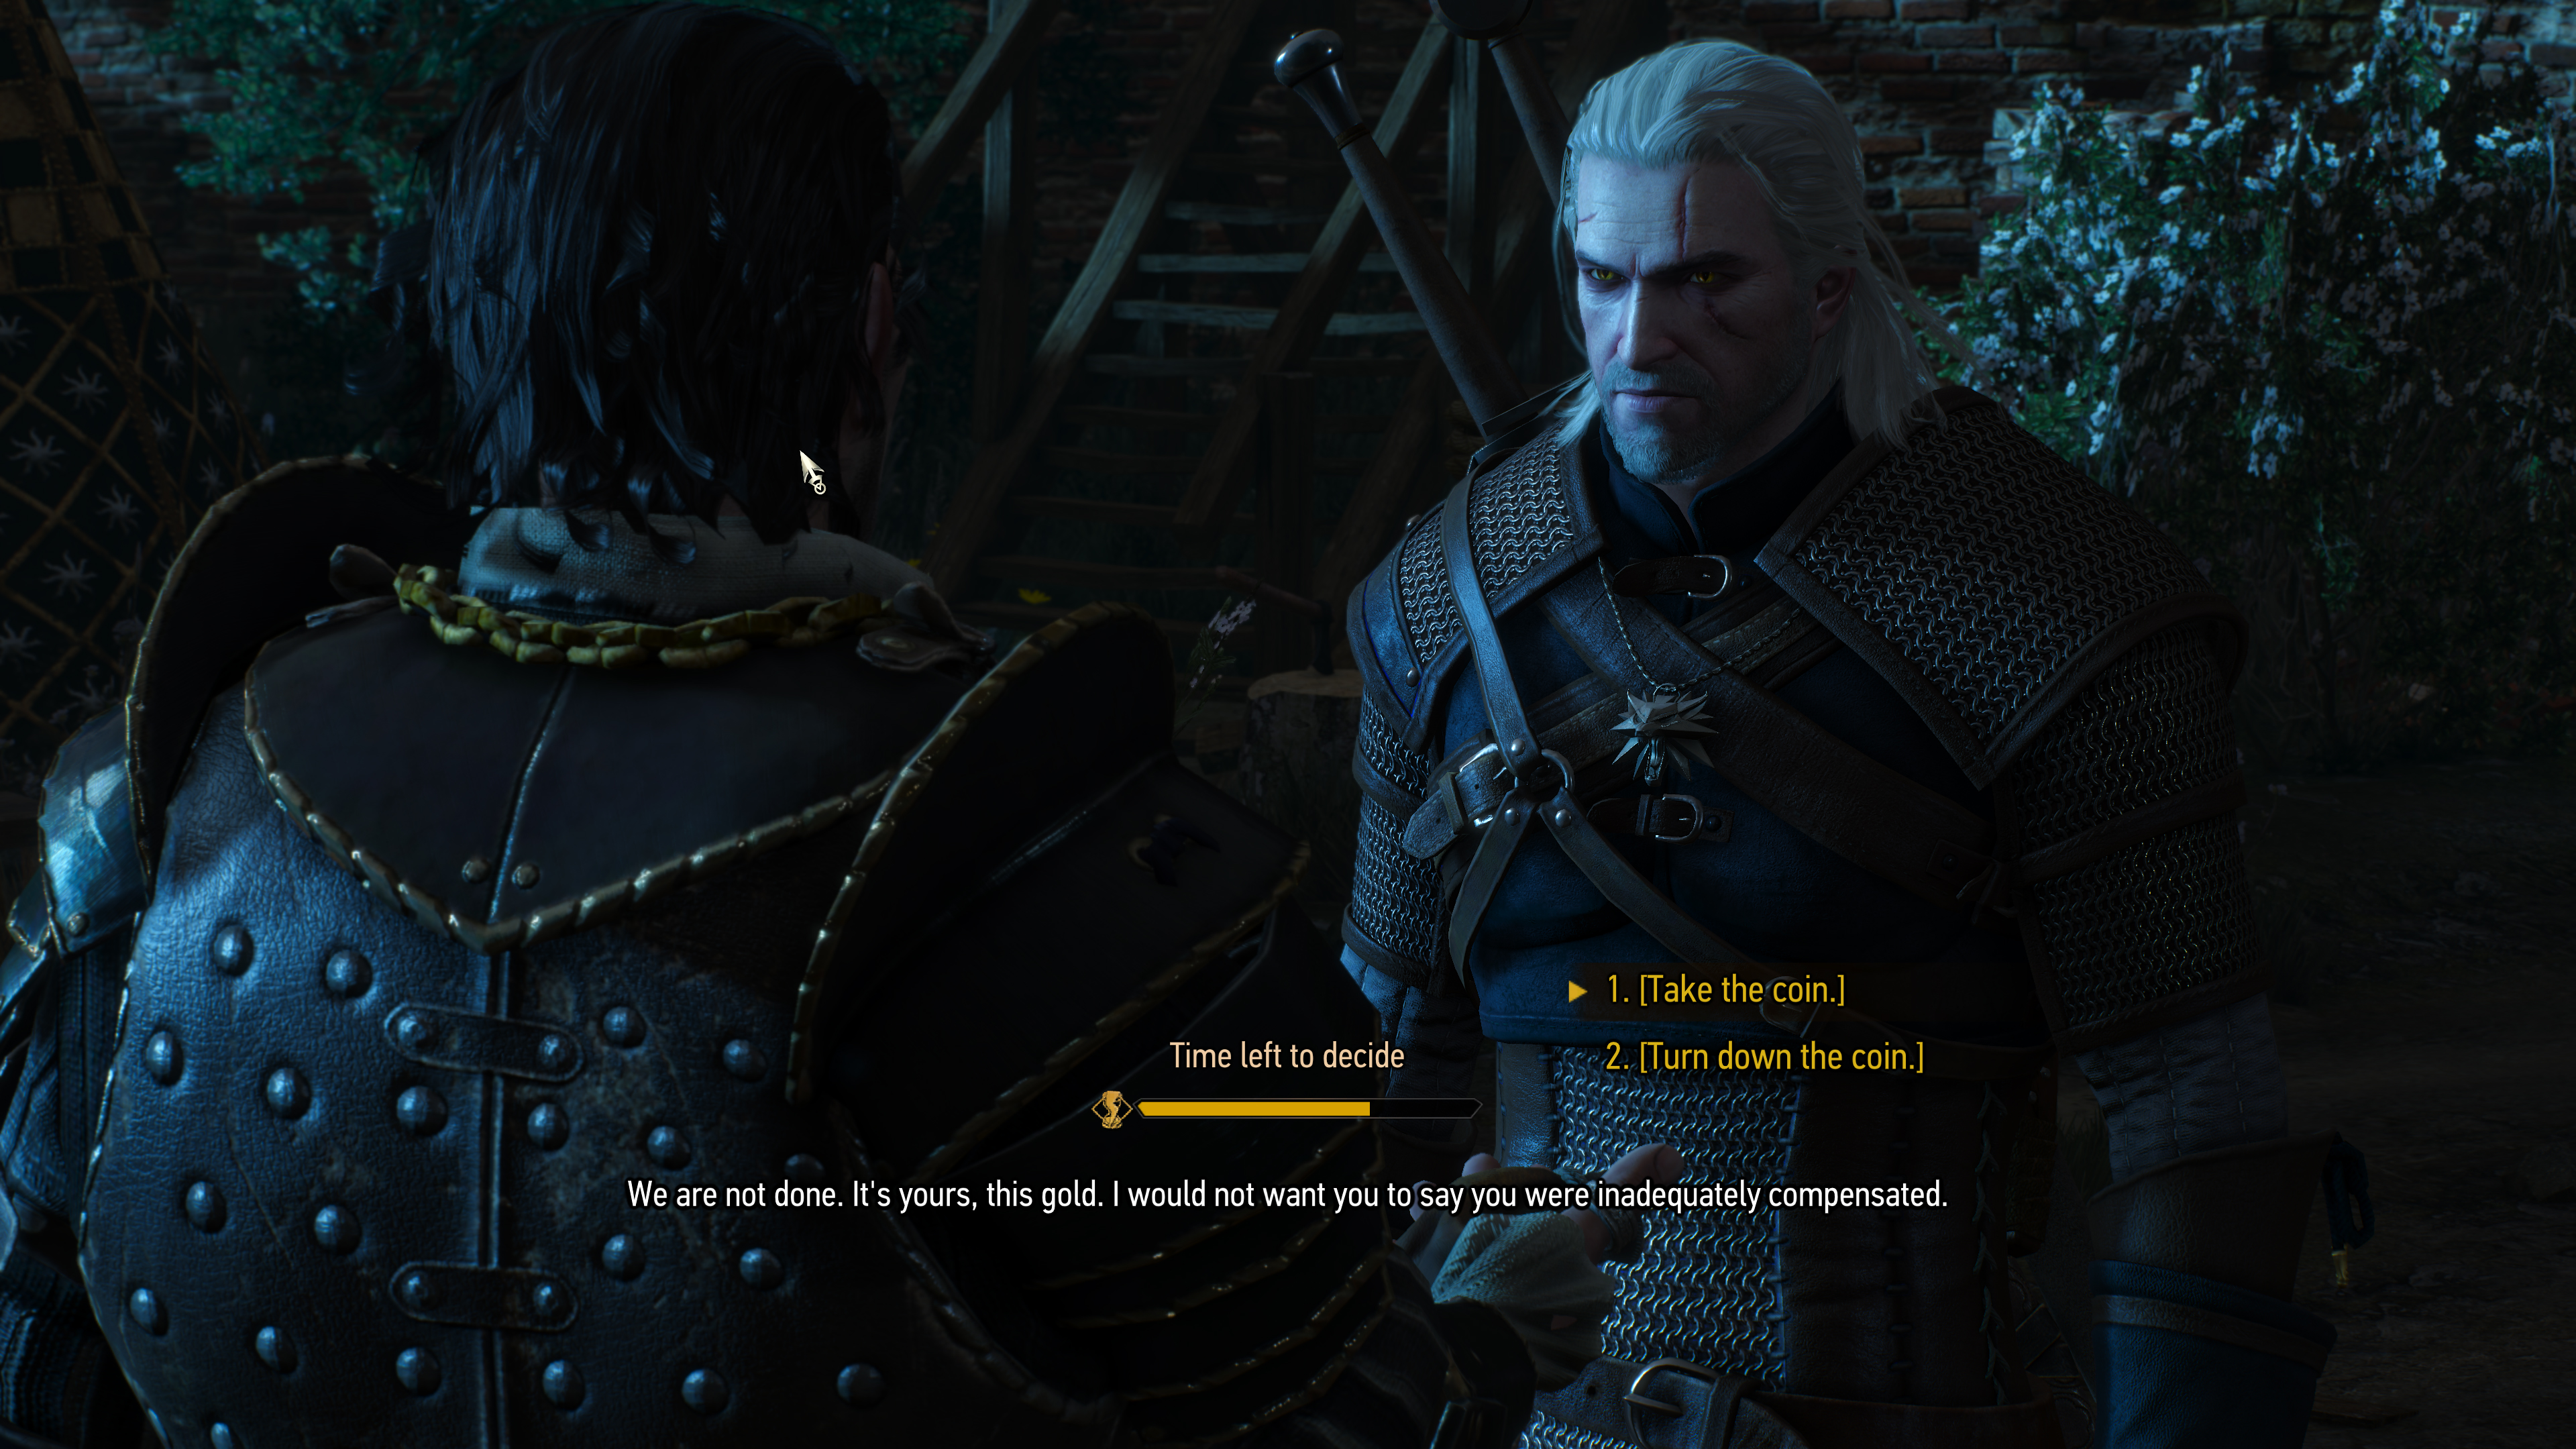
\includegraphics[width=\linewidth, height=6cm]{ch_1_1_2_witcher_2.png}
		\label{subfig:ch_1_1_2_witcher_2}
	\end{subfigure}
	\caption{Wiedźmin 3 (2015)}
	\label{fig:ch1_1_2_witcher}
\end{figure}

\newpage

\subsection{Prześledzenie rozwoju narracji na przykładzie serii Final Fantasy}\label{subsection:ch1_1_3}

% TL;DR:
% - Od FF1 zasadniczo nieme postacie, 2D pikseloza, tylko tekstowe monologi od NPC, cut-scenki bardzo
% prowizoryczne na zasadzie ruszania kamerą w grze. Zero voice actingu i fabuły postaci.
% - Od FF7 pełno-prawna cut-scenka otwarcia, 3D widok, no i chyba bardziej nastawienie na postacie
% - Od FF10 bardzo dużo przerywników filmowych, nastawienie na dialogi, voice acting
% - FF13 historia zeszła na bok w formie dzienniczków, głównie chodzi o dialogi i postacie
% - FF15 jest open world'owe i odeszli od JRPG na rzecz gry akcji

Seria "Final Fantasy" zadebiutowała w 1987 roku na konsoli NES, a samym twórcą gry był Hironobu
Sakaguchi. Na przestrzeni kolejnych lat powstało 14 numerowanych odsłon serii oraz wiele spin-offów
\cite{the_evolution_of_final_fantasy}. W głównej serii każda gra nie miała nic wspólnego z poprzednią
pod względem fabuły, postaci czy uniwersum. Pojawiały się wspólne motywy i stworzenia, ale na ogół
każde "Final Fantasy" stanowiła odrębną, zamkniętą przygodę\cite{the_evolution_of_final_fantasy}.

Seria przeżywała i nadal przeżywa swoistego rodzaju ewolucję narracyjną. Elementy, które stanowiły
główną część fabularną, zeszły na dalszy plan. Początkowo mało istotni bezimienni protagoniści zostali
zastąpieni przez postacie angażujące się w dialogi i rozwijające się na przestrzeni gry
\cite{the_evolution_of_final_fantasy}.

Aby prześledzić proces zmian w serii, dokonany zostanie przegląd kolejnych odsłon "Final Fantasy" na
podstawie informacji zebranych przez Kevin'a Kryah\cite{the_evolution_of_final_fantasy} oraz
Hayes'a Madsen'a\cite{25_years_later}.

W pierwszej odsłonie (Rys. \ref{fig:ch1_1_3_ff1}) fabuła była dość prosta - czterech sterowalnych
bohaterów, znanych jako \textit{Wojownicy Światła}, przybywają do królestwa \textit{Cornelia}, niosąc
mistyczne kule. Zostają poinformowani, że muszą pokonać cztery żywioły, by przywrócić światu równowagę
\cite{the_evolution_of_final_fantasy}. W samej grze \textit{Wojownicy Światła} są niemymi postaciami,
natomiast występują NPC (ang. \textit{non-playable character}), którzy w formie monologów przekazują
graczowi informacje. Monologi te przedstawione są jedynie w formie tekstowej, nie występuje bowiem
zjawisko aktorstwa głosowego (po ang. \textit{voice acting}). Cut-scenki (patrz \ref{subsection:ch1_2_3})
są bardzo prymitywne, na zasadzie poruszania kamerą i wykorzystaniu animacji występujących w grze
(nie są prerenderowane). W ramach ekranu startowego gry przedstawione zostaje graczowi krótkie
wprowadzenie fabularne (Rys. \ref{subfig:ch_1_1_3_ff1_1}).

\begin{figure}[h]
	\begin{subfigure}{0.49\textwidth}
		\caption{Ekran wprowadzający}
		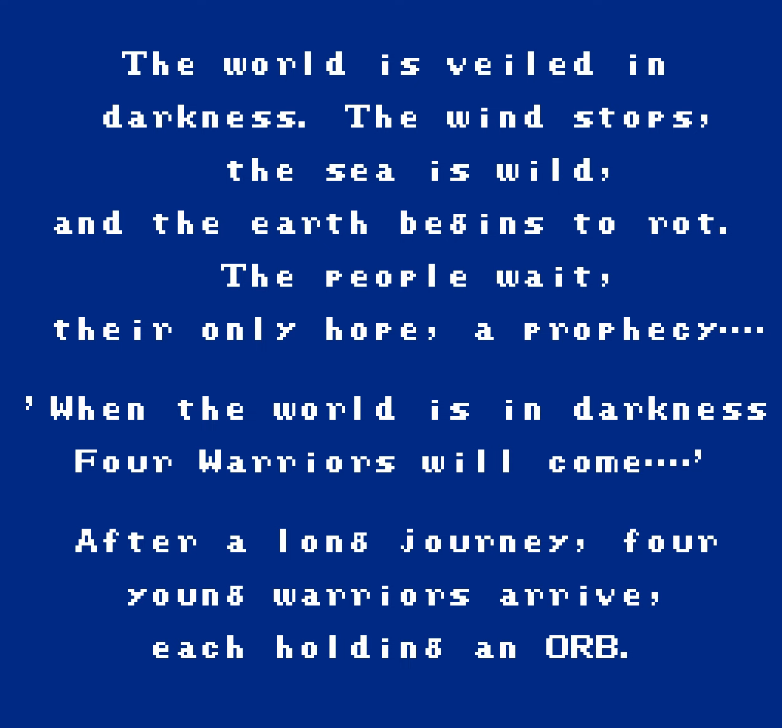
\includegraphics[width=\linewidth, height=6cm]{ch_1_1_3_ff1_1.png}
		\label{subfig:ch_1_1_3_ff1_1}
	\end{subfigure}
	\begin{subfigure}{0.49\textwidth}
		\caption{Rozmowa z NPC}
		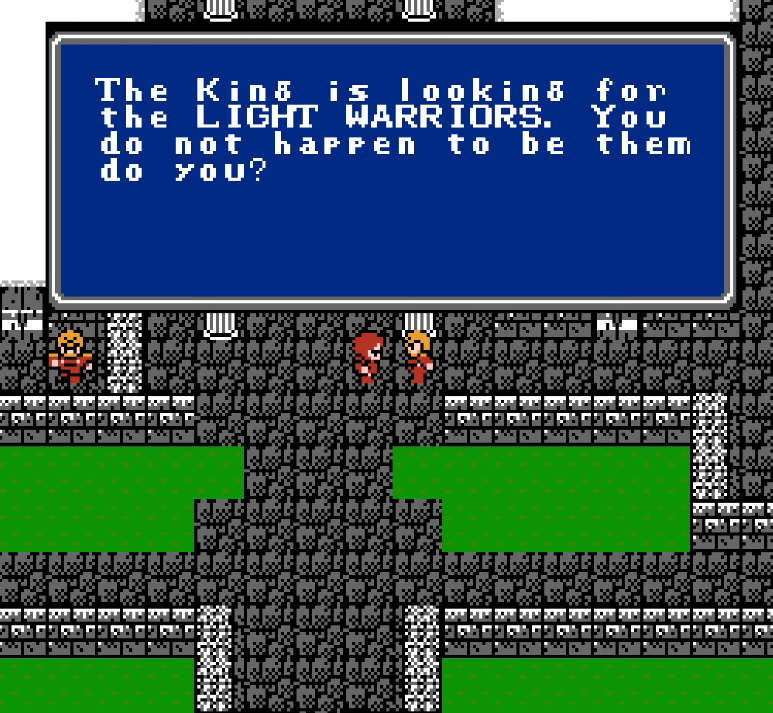
\includegraphics[width=\linewidth, height=6cm]{ch_1_1_3_ff1_2.png}
		\label{subfig:ch_1_1_3_ff1_2}
	\end{subfigure}
	\caption{Final Fantasy I (1987)}
	\label{fig:ch1_1_3_ff1}
\end{figure}

\newpage

Żadne z kolejnych "Final Fantasy" nie wniosły zbyt wiele pod względem złożoności fabuły. "Final Fantasy
IV" wprowadziła większy nacisk na rozwój postaci poprzez cut-scenki i wątki bohaterów. Głównym elementem
nadal pozostawała walka z "ostatecznym złowrogim bossem", lecz przy okazji gracz był w stanie poznać
główne postacie\cite{the_evolution_of_final_fantasy}.

"Final Fantasy VI" poszła o krok dalej - rola postaci zaczęła przesłaniać nadrzędną fabułę. Sceny takie
jak próba samobójcza Celes czy rzut monetą między Edgarem i Sabinem niewiele wniosły do głównego wątku,
ale dobrze charakteryzowały bohaterów w sposób, którego nie sposób opisać samymi dialogami.
\cite{the_evolution_of_final_fantasy}.

W ramach "Final Fantasy VII" (Rys. \ref{fig:ch1_1_3_ff7}) doszło do przełomu graficznego, ponieważ
rozgrywka odbywała się w świecie trójwymiarowym. Dodatkowo, ta część okraszona została pełnoprawną
cut-scenką otwierającą.

"Final Fantasy VII" i VIII kontynuowały trend nastawienia na postaci.
Ich losy stały się głównym tematem, a walka dobra ze złem została odstawiona na dalszy plan.
"Final Fantasy VIII" wydawała się wręcz niezainteresowana głównym wątkiem, a jej zakończenie
koncentrowało się na zamknięciu wątków postaci i zostało zwieńczone pocałunkiem na balkonie
\cite{the_evolution_of_final_fantasy}.

W swej istocie, "Final Fantasy VIII" jest formą opowieści miłosnej. Mimo występowania oczywistych
elementów fantastycznych czy fikcyjnych, to głównym motywem przyciągającym uwagę gracza jest
miłość Squalla i Rinoi\cite{25_years_later}.

Hayes Madsen sugeruje, iż to właśnie przez występowanie takich osobistych historii czy relacji między
postaciami fabuła "Final Fantasy VIII" jest tak często wspominana. Twórcy przedstawili bowiem występujące
pomiędzy głównymi postaciami poczucie koleżeństwa i ich wspólnego rozwoju\cite{25_years_later}.

\begin{figure}[h]
	\begin{subfigure}{0.49\textwidth}
		\caption{Klatka cut-scenki wprowadzającej}
		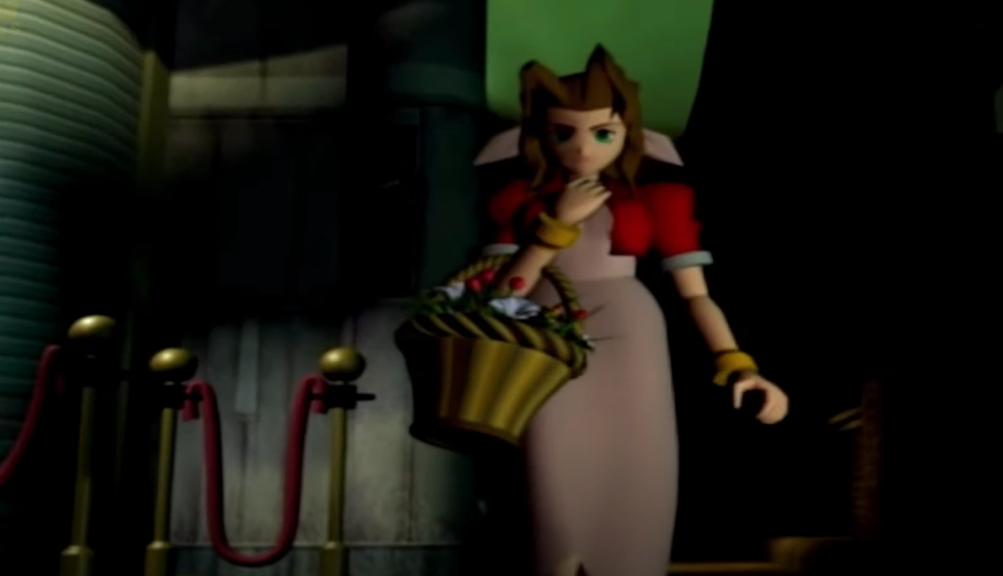
\includegraphics[width=\linewidth, height=6cm]{ch_1_1_3_ff7_1.png}
		\label{subfig:ch_1_1_3_ff7_1}
	\end{subfigure}
	\begin{subfigure}{0.49\textwidth}
		\caption{Dialogi pomiędzy postaciami}
		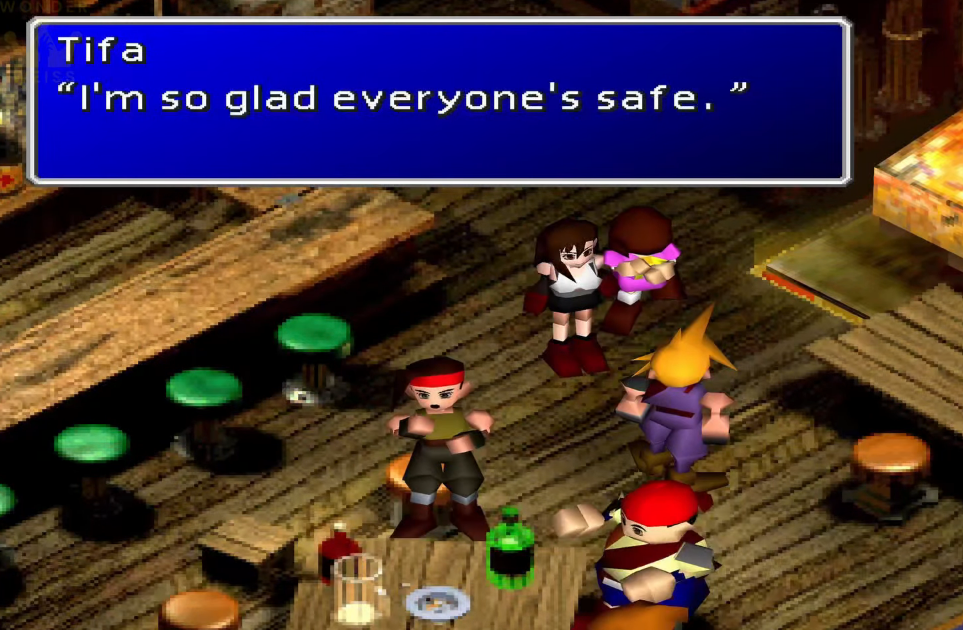
\includegraphics[width=\linewidth, height=6cm]{ch_1_1_3_ff7_2.png}
		\label{subfig:ch_1_1_3_ff7_2}
	\end{subfigure}
	\caption{Final Fantasy VII (1997)}
	\label{fig:ch1_1_3_ff7}
\end{figure}

\newpage

Gdy seria wkroczyła w XXI wiek, gry oddalały się jeszcze bardziej od swych korzeni. "Final Fantasy
IX" kontynuowała nastawienie na postacie, dodając klimat europejskich baśni czy aluzji do Szekspira i
Carrolla. "Final Fantasy X" (Rys. \ref{fig:ch1_1_3_ff10}) podejmowała tematy religii i człowieczeństwa,
prezentując jednocześnie jedne z najbardziej artystycznych wizji w serii\cite{the_evolution_of_final_fantasy}.
Rozgrywka została urozmaicona bardzo wieloma zaawansowanymi przerywnikami filmowymi. Postacie wydawać się
mogą zdecydowanie bardziej realistyczne czy "żywsze" ze względu na udział aktorów głosowych, począwszy
od tej części.

\begin{figure}[h]
	\begin{subfigure}{0.49\textwidth}
		\caption{Cut-scenka z gry}
		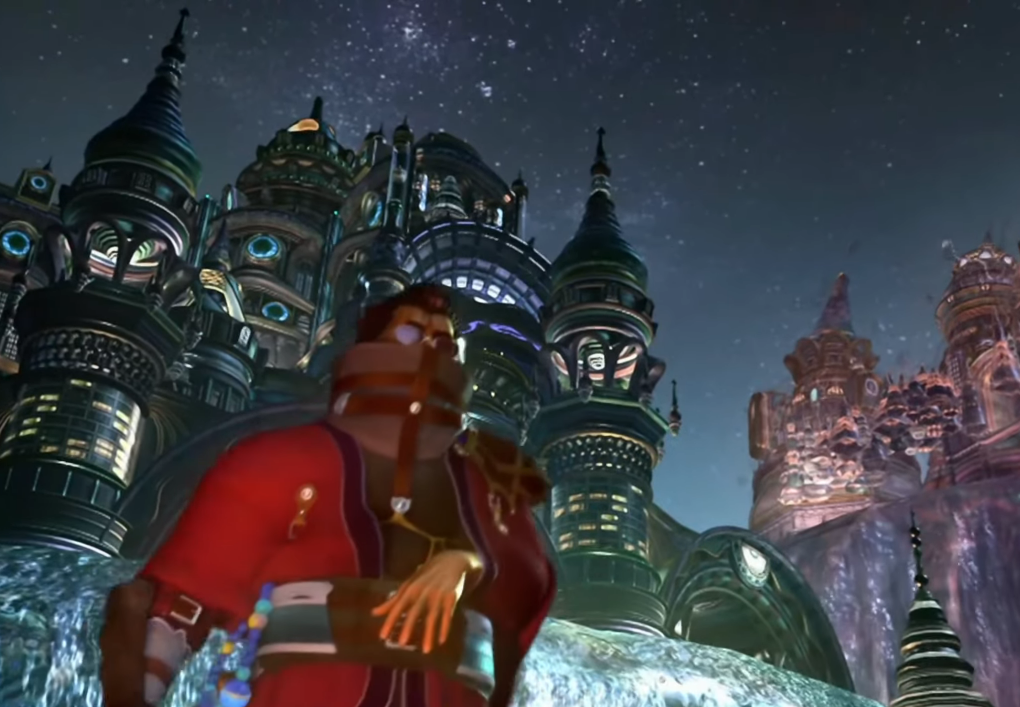
\includegraphics[width=\linewidth, height=6cm]{ch_1_1_3_ff10_1.png}
		\label{subfig:ch_1_1_3_ff10_1}
	\end{subfigure}
	\begin{subfigure}{0.49\textwidth}
		\caption{Dialogi pomiędzy postaciami}
		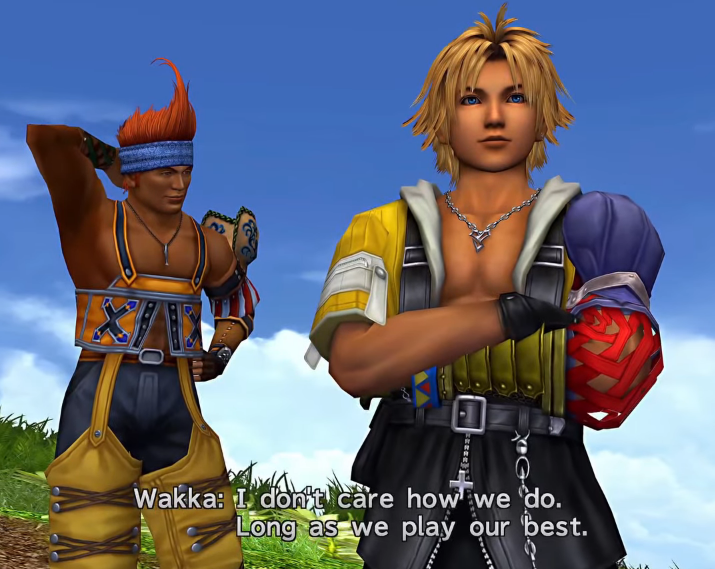
\includegraphics[width=\linewidth, height=6cm]{ch_1_1_3_ff10_2.png}
		\label{subfig:ch_1_1_3_ff10_2}
	\end{subfigure}
	\caption{Final Fantasy X (2001)}
	\label{fig:ch1_1_3_ff10}
\end{figure}

\newpage

"Final Fantasy XIII" (Rys. \ref{fig:ch1_1_3_ff13}) w pełni skupiło się na rozwoju postaci i
formie wizualnej, natomiast sensowność fabuły pozostawiała wiele do życzenia. W rzeczywistości większość
istotnych informacji nie jest dostarczana w dialogach, ale za pośrednictwem wpisów do dziennika,
znajdywanych przez gracza w trakcie rozgrywki. To raczej postacie zajęły centralne miejsce, a
bezsensowna fabuła starała się jedynie związać ze sobą wszystkie wątki
bohaterów\cite{the_evolution_of_final_fantasy}.

\begin{figure}[h]
	\begin{subfigure}{0.49\textwidth}
		\caption{zzz}
		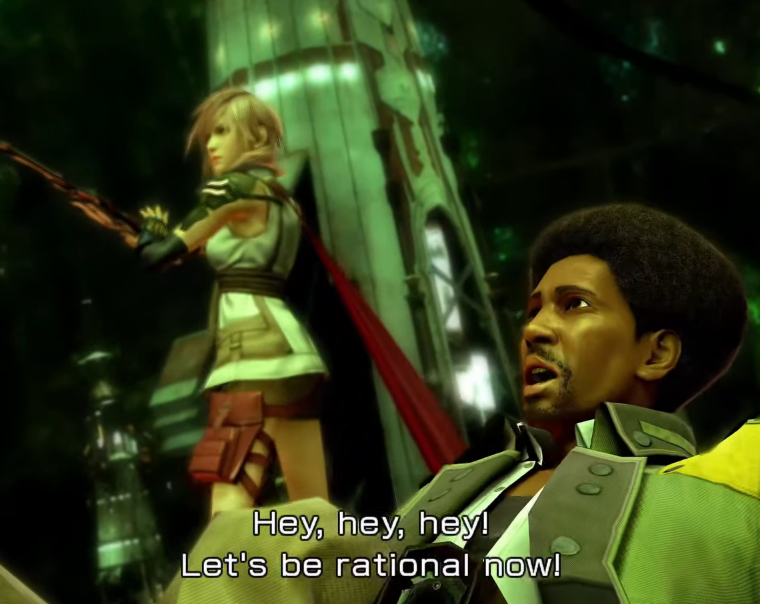
\includegraphics[width=\linewidth, height=6cm]{ch_1_1_3_ff13_1.png}
		\label{subfig:ch_1_1_3_ff13_1}
	\end{subfigure}
	\begin{subfigure}{0.49\textwidth}
		\caption{zzz}
		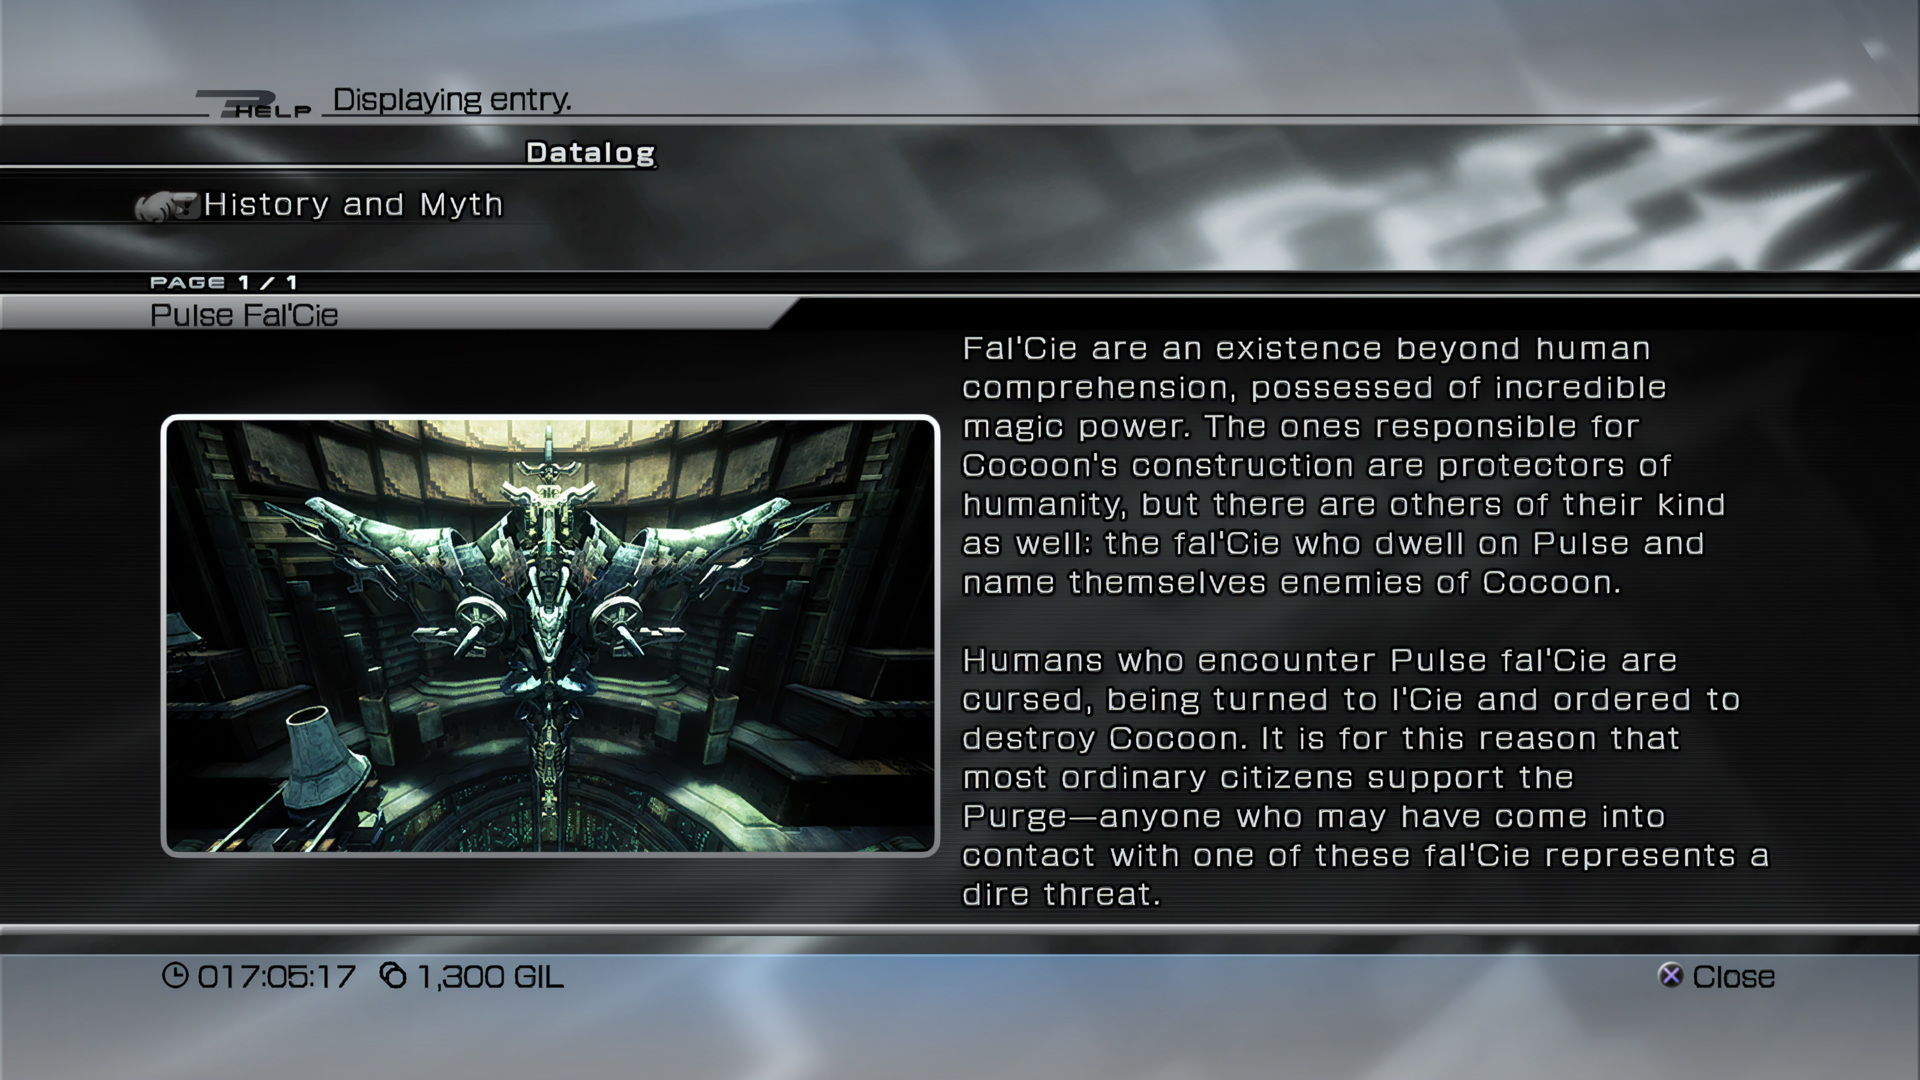
\includegraphics[width=\linewidth, height=6cm]{ch_1_1_3_ff13_2.png}
		\label{subfig:ch_1_1_3_ff13_2}
	\end{subfigure}
	\caption{Final Fantasy XIII (2009)}
	\label{fig:ch1_1_3_ff13}
\end{figure}

Seria "Final Fantasy" rozwija się po dzień dzisiejszy, a twórcy nadal próbują używać różnych rozwiązań by
wyróżnić kolejne tytuły. Przykładowo, w najnowszej odsłonie serii --- "Final Fantasy XV" --- deweloperzy
odeszli od konwencji JRPG (ang. \textit{Japanese role-playing game}) na rzecz gry akcji z otwartym światem.

Na przestrzeni lat seria "Final Fantasy" przeszła znaczącą ewolucję pod względem roli i znaczenia narracji.
Niezależnie od zmian w strukturze rozgrywki czy sposobie prezentowania fabuły, widoczny jest stale rosnący
wpływ elementów narracyjnych na całokształt kolejnych odsłon serii.

\newpage

\section{Rodzaje narracji w grach komputerowych}\label{section:ch1_2}

Poniższa sekcja ma na celu uporządkowanie --- znanych z literatury czy też istniejących
przykładów --- struktur narracyjnych, za pomocą których opisać można sekwencję kolejnych
wydarzeń w grze. Dodatkowo, przedstawione zostaną kluczowe sposoby czy też techniki, za
pomocą których twórcy budują wirtualne światy fabularne.

\subsection{Struktury narracyjne}\label{subsection:ch1_2_1}

Pod pojęciem \textit{struktury narracyjnej} rozumiane jest \textbf{uporządkowanie}
wydarzeń odbywających się w grze, które niosą jakiekolwiek przesłanki fabularne.
Nie oznacza to, że każde wydarzenie musi się odbyć --- może być to bowiem zależne od
decyzji podjętych przez grającego. Wyszczególnione zostaną trzy klasyczne struktury,
które zapewniają dość płynny przebieg historii, a są to: \textit{liniowa}, \textit{łańcuch pereł},
\textit{rozgałęziającą się}\cite{the_evolution_of_video_games}\cite{theorising_narrative}\cite{narrative_structures}.
Z zakresu mniej oczywistych architektur dodatkowo warto wspomnieć o modelach
\textit{parku rozrywki} i \textit{cegiełek}\cite{theorising_narrative}.

\subsubsection*{Liniowa}

Jest to forma przekazu znana bardzo dobrze z literatury czy też kinematografii. Sprowadza się ona
bowiem do jednego ciągu zdarzeń, gdzie odbiorca nie ma wpływu na dalszy przebieg fabuły lecz jest
on raczej pasywnym obserwatorem odgrywających się scen. W przypadku książki czy filmu jest to
naturalne podejście ze względu na brak interaktywności. Jeśli chodzi o gry komputerowe, to
strukturę tą można zaobserwować zwłaszcza w \textit{"starszych"} tytułach (Np. wspomniany wcześniej
"Crash Bandicoot" - patrz \ref{subsection:ch1_1_2}). Gra zasadniczo może być ukończona na jeden
sposób --- tak jak to zaplanowali projektanci\cite{the_evolution_of_video_games} (Patrz Rys. \ref{fig:ch1_2_1_linear}).

\begin{figure}[h]
	\caption{Liniowa struktura gry\cite{narrative_structures}}
	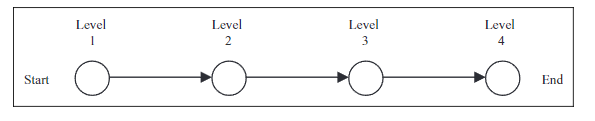
\includegraphics[width=\textwidth]{ch_1_2_1_linear.png}
	\centering
	\label{fig:ch1_2_1_linear}
\end{figure}

\subsubsection*{Łańcuch pereł}

W ramach tego modelu gracze uzyskują pewnego rodzaju \textit{"iluzję"} wyboru. Występują podczas
rozgrywki momenty swobody, gdzie grający mają poczucie wpływu na dalszy przebieg fabularny. W
rzeczywistości jednak podejmowane przez nich decyzje mogą nie posuwać historii na przód, a same
postępy narracyjne nadal znajdują się pod kontrolą projektantów gry\cite{theorising_narrative}.
Tak jak przedstawiono na rysunku \ref{fig:ch1_2_1_pearls} --- mogą występować tymczasowe rozgałęzienia
wychodzące od głównej sekwencji fabularnej, natomiast zostają one w końcu urwane, a gracz zobowiązany
jest do kontynuowania przygody według zaplanowanej historii. Jako przykład może służyć "The Legend
of Zelda" (Patrz \ref{subsection:ch1_1_2}), gdzie grający może zwiedzać dane poziomy w dość dowolny
sposób, natomiast musi ostatecznie trafić na główną ścieżkę by móc dokonać postępu.

\begin{figure}[h]
	\caption{Struktura łańcuchu pereł}
	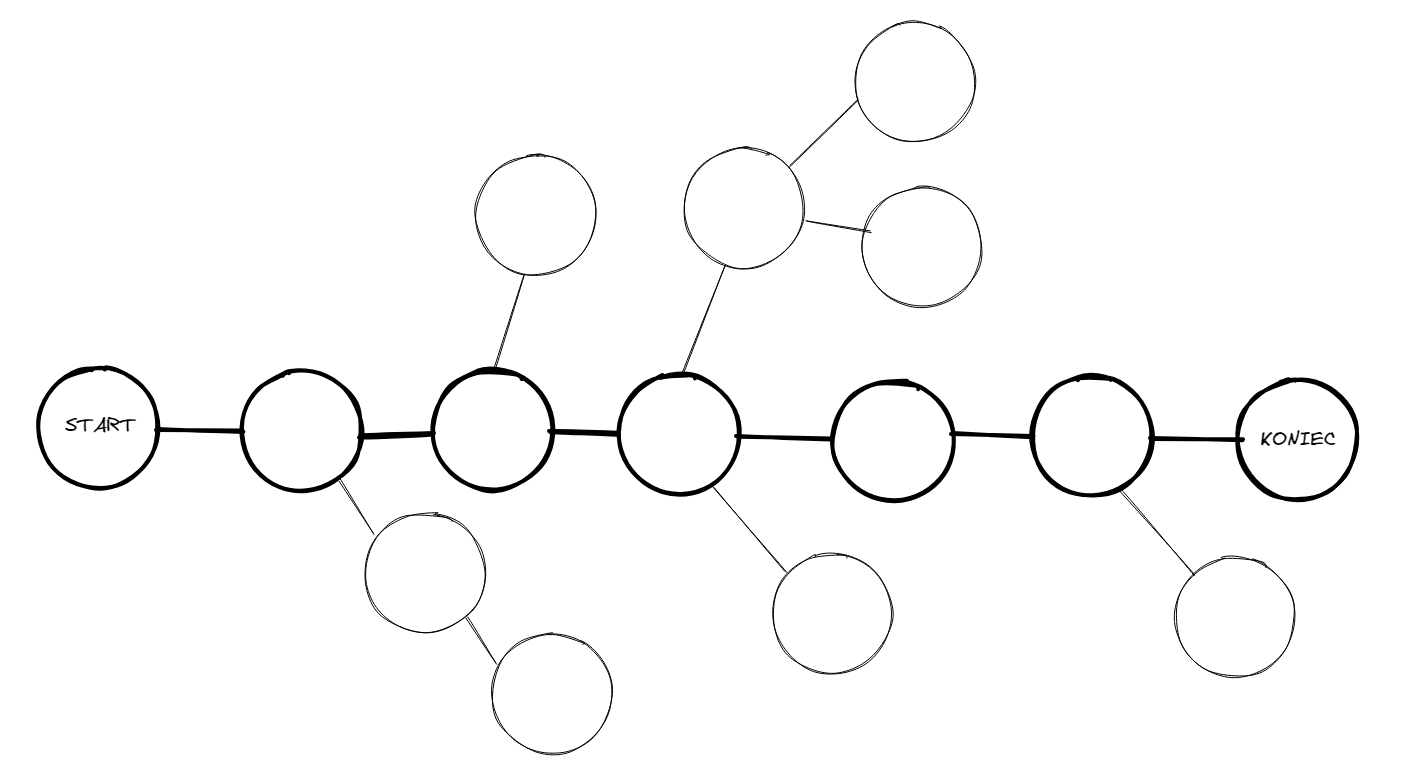
\includegraphics[width=\textwidth]{ch_1_2_1_pearls.png}
	\centering
	\label{fig:ch1_2_1_pearls}
\end{figure}

\subsubsection*{Rozgałęziająca się}

Metodą, która oferuje graczowi istotny wpływ na przebieg dalszej rozgrywki jest zdecydowanie
model rozgałęziający się. Jak sama nazwa wskazuje, historia nie trzyma się jednej konkretnej wersji
lecz jest w stanie \textit{"rozgałęziać się"} w wielu innych możliwych kierunkach. Może to wynikać
z jawnych decyzji podejmowanych przez gracza w istotnych momentach lub też ze względu na sposób
w jaki podchodzi on do rozgrywki (np. może pomijać pewne elementy świata)\cite{theorising_narrative}.
W wyniku takich rozgałęzień wytwarza się pewnego rodzaju "sieć możliwości fabularnych"\cite{theorising_narrative}
--- które z reguły muszą być uprzednio przygotowane przez projektantów gry. Struktura ta została
przedstawiona na rysunku \ref{fig:ch1_2_1_branching} --- akcja zaczyna się w jednym punkcie, potem
w wyniku decyzji istniejących w grze występują rozgałęzienia, które ostatecznie prowadzą do potencjalnie
różnych zakończeń (oznaczonych czerwonymi rombami). Przykładem realizującym ten model może być
wspomniany wcześniej tytuł "Life is Strange" (Patrz \ref{subsection:ch1_1_2}).

\begin{figure}[h]
	\caption{Struktura rozgałęziająca się}
	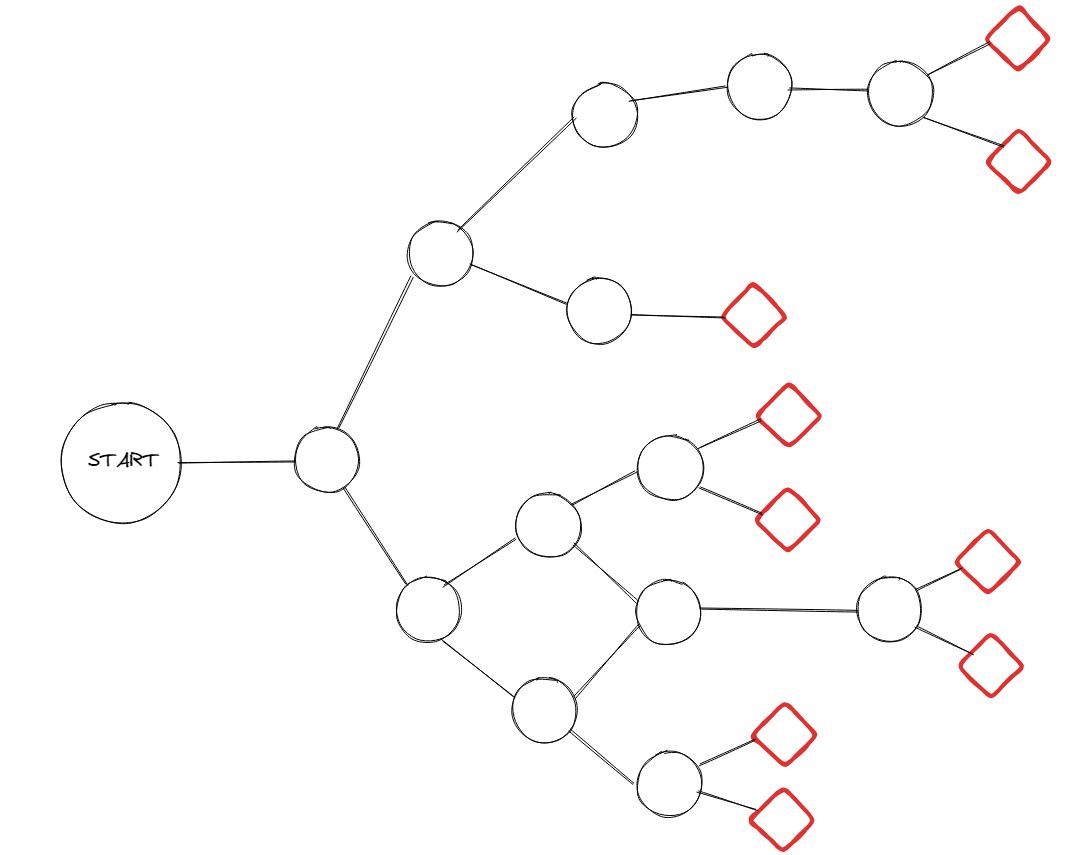
\includegraphics[width=\textwidth]{ch_1_2_1_branching.png}
	\centering
	\label{fig:ch1_2_1_branching}
\end{figure}

\newpage

\subsubsection*{Park rozrywki}

Struktura ta z założenia bardzo przypomina model rozgałęziający się, natomiast w tym przypadku
możemy mówić o narracji rozwijającej się ze względu na przestrzeń a nie czas\cite{theorising_narrative}.
Przykładowo, zwiedzając świat gry gracz może napotkać postać NPC, która otworzy przed nim nową
gałąź fabularną (np. poprzez zlecenia zadania do wykonania)\cite{the_evolution_of_video_games}.
Model ten jest bardzo popularny dla gier z otwartym światem, przykładem może być "Wiedźmin 3"
(Patrz \ref{subsection:ch1_1_2}).

\subsubsection*{Cegiełki}

W ramach niektórych tytułów twórcy nie skupiają się na stworzeniu narracji możliwej do doświadczenia
przez grającego, lecz na pewnym systemie części, za pomocą których gracz sam jest w stanie tworzyć
historię. Części te nazywane \textit{"cegiełkami"} (ang. \textit{building blocks})\cite{theorising_narrative}
są wykorzystywane przez grającego do tworzenia własnej narracji. Przykładem tego rodzaju rozgrywki
może być tytuł "The Sims" (2000), w którym to gracz tworzy i steruje rodziną --- a co za tym idzie,
kieruje ich historią życia.

\subsection{Sposoby przedstawiania narracji}\label{subsection:ch1_2_2}

No ogólnie narrację można przedstawiać na różne sposoby wiadomo mhm mhm

\begin{itemize}
	\item Cut-scenki
	\item Tekst (elementy interfesju, bloki do czytania)
	\item Dialogi (z NPC)
	\item Poprzez świat gry (audio-wizualnie)
\end{itemize}

\newpage

\section{Systemy dialogowe w grach komputerowych}\label{section:ch1_3}

fefef

\subsection{Popularne systemy dialogowe}\label{subsection:ch1_3_1}

fefef

\subsection{Interaktywna fikcja - system poleceń}\label{subsection:ch1_3_2}

ortatraoitrmoi